\PassOptionsToPackage{utf8}{inputenc}
\documentclass{bioinfo}
\copyrightyear{2015} \pubyear{2015}

\access{Advance Access Publication Date: Day Month Year}
\appnotes{Manuscript Category}



%%% PACKAGES
\usepackage{booktabs} % for much better looking tables
\usepackage{array} % for better arrays (eg matrices) in maths
\usepackage{paralist} % very flexible & customisable lists (eg. enumerate/itemize, etc.)
  \let\itemize\compactitem
  \let\enditemize\endcompactitem
  \let\enumerate\compactenum
  \let\endenumerate\endcompactenum
  \let\description\compactdesc
  \let\enddescription\endcompactdesc
  \pltopsep=1pt
  \plitemsep=1pt
  \plparsep=1pt  
\usepackage{hyperref} 
\usepackage{xspace} 
\usepackage{amsmath,amssymb} 
\usepackage{bm}
\usepackage{verbatim}
\usepackage{longtable}
\usepackage[vlined]{algorithm2e}

%%%%%%%%%%%%%%%%%%%%%%%%%%%%%%%%%%%%%%%%
%% Rolf's includegraphicstop
\makeatletter
\newsavebox{\@alignepsbox}
\newlength{\@aligneps}
\newcommand{\includegraphicstop}[2][]{%
\sbox{\@alignepsbox}{\includegraphics[#1]{#2}}%
\setlength{\@aligneps}{-\ht\@alignepsbox}%
\addtolength{\@aligneps}{2ex}%
\raisebox{\@aligneps}{\usebox{\@alignepsbox}}}
\makeatother


\makeatletter
\let\oldlt\longtable
\let\endoldlt\endlongtable
\def\longtable{\@ifnextchar[\longtable@i \longtable@ii}
\def\longtable@i[#1]{\begin{figure}[t]
\onecolumn
\begin{minipage}{0.5\textwidth}
\oldlt[#1]
}
\def\longtable@ii{\begin{figure}[t]
\onecolumn
\begin{minipage}{0.5\textwidth}
\oldlt
}
\def\endlongtable{\endoldlt
\end{minipage}
\twocolumn
\end{figure}}
\makeatother

%%%%%%%%%%%%%%%%% Theorems %%%%%%%%%%%%%%%%%%%%%%%%%

 \newtheorem{theorem}{Theoreme}
 \newtheorem{definition}[theorem]{Definition}
 \newtheorem{remark}[theorem]{Remark}
 \newtheorem{corollary}[theorem]{Corollary}
 \newtheorem{lemma}[theorem]{Lemma}
 \newtheorem{proposition}[theorem]{Proposition}

\newtheorem{observation}[theorem]{Observation}

%\newtheorem{algorithm}{Algorithm}
\newtheorem{axiom}{Axiom}
\newtheorem{hypothesis}{Working Hypothesis}

%%% macros for notation in DP framework
\newcommand{\network}{\mathcal{N}}
\newcommand{\dom}{\operatorname{dom}} %domain
\newcommand{\val}{a} % valuation aka assignment
\newcommand{\vars}{\operatorname{vars}}
\newcommand{\dep}{\operatorname{dep}}
\newcommand{\energy}[1]{\operatorname{e}_{#1}}
\newcommand{\numberof}{\operatorname{\#}}
\newcommand{\partfun}[1]{\mathcal{Z}_{#1}}
\newcommand{\separator}[2]{\operatorname{sep}(#1,#2)}
\newcommand{\difference}[2]{\operatorname{diff}(#1 \rightarrow #2)}
\newcommand{\real}{\mathbb{R}}
\newcommand{\genmarg}[1]{(\!|\!#1\!|\!)}
\newcommand{\gencomb}[1]{\langle\!|#1|\!\rangle}
\newcommand{\Message}[2]{m_{#1\rightarrow #2}}


\newcommand{\energyModel}{{\cal M}}
\newcommand{\structureElements}{{\cal SE}}
\newcommand{\powerSet}[1]{2^{#1}}
\newcommand{\underConstruction}[1]{{\LARGE$\triangle$\Large\!\!\!\!!}$\quad$\textcolor{red}{#1}}
\newcommand{\argmin}{\operatorname*{arg\,min}}
\newcommand{\objective}{{\mathbb{F}}}

%\newcommand{\assignments}{\operatorname{as}}
\newcommand{\assignments}{\mathcal{A}}
\newcommand{\B}{\mathcal{B}}
\newcommand{\F}{\mathcal{F}}
\newcommand{\I}{\mathcal{I}}
\newcommand{\R}{\mathcal{R}}
\renewcommand{\S}{\mathcal{S}}
\newcommand{\X}{\mathcal{X}}
\newcommand{\Y}{\mathcal{Y}}

\newcommand{\width}{w}

\newcommand{\sample}{\texttt{Sample}}
\newcommand{\elim}[2]{\operatorname{elim}(#1,#2)}
\newcommand{\edgesToR}{E^r_T}

\newcommand{\phitotal}{\phi_{\operatorname{m}}}

\newcommand{\Ebp}[2]{E^{\textrm{bp}}_{#1}(#2)}
\newcommand{\Ehp}[1]{E^{\textrm{hp}}(#1)}
\newcommand{\Eint}[1]{E^{\textrm{int}}(#1)}

\newcommand{\Def}[1]{{\bf #1}}

\newcommand{\TargetE}{E^{\star}}



\newcommand{\TODO}[1]{\Final{\begin{mdframed}[leftline=false,rightline=false,linecolor=red!70!black,linewidth=1.5pt]\color{red!70!black}\sf TODO: #1\end{mdframed}}}
\newcommand{\parHead}[1]{\Final{\paragraph{#1}}}


\newcommand{\Final}[1]{#1}
%% Uncomment the line below for ``Final'' version
\renewcommand{\Final}[1]{}

\newcommand{\Design}[1]{{\sf Designs}^{\star}(#1)}
\newcommand{\NumDesign}{\ensuremath{\#}{\sf Designs}\xspace}
\newcommand{\IS}[1]{{\sf IndSets}(#1)}
\newcommand{\Nuc}[1]{{\sf #1}}
\newcommand{\Ab}{\Nuc{A}}
\newcommand{\Cb}{\Nuc{C}}
\newcommand{\Gb}{\Nuc{G}}
\newcommand{\Ub}{\Nuc{U}}

\newcommand{\Software}[1]{{\ttfamily #1}}

\newcommand{\ourprog}{\Software{RNARedPrint}}

\setlength{\parskip}{.2em}



%%% end macro defs



\begin{document}
\firstpage{1}

\subtitle{Subject Section}

\title[short Title]{Fixed-Parameter Tractable Sampling for RNA Design with Multiple Target Structures}
\author[Hammer, Ponty, Wang and Will]{Stefan Hammer\,$^{\text{\sfb 1,2,3}}$, Yann Ponty\,$^{\text{\sfb 4,5,}\star}$, Wei Wang\,$^{\text{\sfb 4}}$ and Sebastian Will\,$^{\text{\sfb 2}}$}
\address{$^{\text{\sf 1}}$University Leipzig, Department of Computer Science and Interdisciplinary Center for Bioinformatics, 04107 Leipzig, Germany; 
$^{\text{\sf 2}}$University of Vienna, Faculty of Chemistry, Department of Theoretical Chemistry, 1090 Vienna, Austria;
$^{\text{\sf 3}}$University of Vienna, Faculty of Computer Science, Research Group Bioinformatics and
Computational Biology, 1090 Vienna, Austria;
$^{\text{\sf 4}}$CNRS UMR 7161 LIX, Ecole Polytechnique, Bat. Turing, 91120 Palaiseau, France;
and $^{\text{\sf 5}}$ AMIBio team, Inria Saclay, Bat Alan Turing, 91120 Palaiseau, France}

\corresp{$^\ast$To whom correspondence should be addressed.}

\history{Received on XXXXX; revised on XXXXX; accepted on XXXXX}

\editor{Associate Editor: XXXXXXX}

\abstract{\textbf{Motivation:} The design of multi-stable RNA molecules has important applications in biology, medicine, and biotechnology. Synthetic design approaches largely benefit from effective in-silico methods, which can tremendously impact their cost and feasibility. \\
\textbf{Results:} Here, we revisit a central ingredient of most in-silico design methods: the sampling of sequences for multi-target design. We establish the $\#${\sf P}-hardness of uniform sampling, and introduce \ourprog{}, a tree decomposition-based algorithm for efficient, fixed parameter tractable sampling. By modeling the problem as a constraint network, \ourprog{} supports generic Boltzmann-weighted sampling for arbitrary additive RNA energy models; this enables generating designs meeting specific goals like expected free energies or \Gb\Cb-content. Finally, we empirically study general properties of the approach and generate biologically relevant multi-target Boltzmann-weighted designs for a common design benchmark. In particular, we show significant improvements over seed sequences generated by uniform sampling, the previously best available sampling strategy for multi-target design.\\
\textbf{Availability:} \url{https://github.com/yannponty/RNARedPrint}\\
\textbf{Contact:} Our software is freely available at: \href{yann.ponty@lix.polytechnique.fr}{yann.ponty@lix.polytechnique.fr}\\
\textbf{Supplementary information:} Supplementary data are available at \textit{Bioinformatics}
online.}

\maketitle



\section{Introduction}
\parHead{Design, applications and motivation for multiple design.}Synthetic biology endeavors the engineering of artificial biological
systems, promising broad applications in biology, biotechnology and
medicine. Centrally, this requires the design of biological
macromolecules with highly specific properties and programmable functions.
In particular, RNAs present themselves as well-suited tools for
rational design targeting specific functions~\cite{Kushwaha2016}. RNA function is tightly
coupled to the formation of secondary structure, as well as changes in
base pairing propensities and the accessibility of regions, e.g. by
burying or exposing interaction sites~\cite{Rodrigo2014}. At the same time, the
thermodynamics of RNA secondary structure is well understood and its prediction is
computationally tractable~\cite{McCaskill1990}. Thus,  structure can serve as effective
proxy within rational design approaches, ultimately targeting catalytic~\cite{Zhang2013} or regulatory~\cite{Rodrigo2014} functions.

\parHead{Motivating multiple RNA design.} The function of many RNAs
depends on their selective folding into one or several alternative
conformations. Classic examples include riboswitches, which
notoriously adopt different stable structures upon binding a specific
ligand. Riboswitches have been a popular application of rational
design~\cite{Wachsmuth2013,Domin2017}, partly motivated by their capacity to
act as biosensors~\cite{Findeiss2017}. At the co-transcriptional
level, certain RNA families feature alternative, evolutionarily
conserved, transient structures~\cite{Zhu2013}, which facilitate the
ultimate adoption of functional structures at full elongation.  More
generally, simultaneous compatibility to multiple structures
is a relevant design objective for engineering kinetically controlled RNAs, finally targeting prescribed folding pathways. Thus,
modern applications of RNA design often target (the simultaneous
stability of) multiple structures, additionally aiming at other
features, such as specific \Gb\Cb-content~\cite{Reinharz2013} or the
presence/absence of functionally relevant motifs (either anywhere or
at specific positions)~\cite{Zhou2013}; these objectives motivate flexible
computational design methods.

\parHead{On the importance of sampling for design.}
Many computational methods for RNA design rely on similar overall
strategies: initially generating one or several \Def{seed} sequences
and optimizing them subsequently. In many cases, the seed quality was
found to be critical for the empirical performance (and solution
quality) of RNA design methods~\cite{Levin2012}. For instance, random
seed generation improves the prospect of subsequent optimizations, helping
to overcome local optima of the objective function, and induce better
sequence diversity across designs~\cite{Reinharz2013}.  For
single-target approaches, \Software{INFO-RNA}~\cite{Busch2006} made
significant improvements mainly by starting its local search from the
minimum energy sequence for the target structure instead of (uniform)
random sequences for the early \Software{RNAinverse}
algorithm~\cite{Hofacker1994}. This strategy was later shown to result
in unrealistically high \Gb\Cb-contents in designed sequences. To
address this issue, \Software{IncaRNAtion}~\cite{Reinharz2013}
controls the \Gb\Cb-content through an adaptive sampling strategy.

\parHead{Specificities and similarities of multi-target design.}
Specifically, for multi-target design, virtually all available methods~\cite{Lyngsoe2012,HoenerzuSiederdissen2013,Taneda2015,Hammer2017} follow the same overall generation/optimization scheme.
%
Facing the complex sequence constraints induced by multiple targets, early methods such as \Software{Frnakenstein}~\cite{Lyngsoe2012} and \Software{Modena}~\cite{Taneda2015} did not attempt to solve sequence generation systematically, but rely on \emph{ad-hoc} sampling strategies. 
%
Recently, the \Software{RNAdesign} approach~\cite{HoenerzuSiederdissen2013}, coupled with powerful local search within \Software{RNAblueprint}~\cite{Hammer2017}, solved the problem of sampling seeds from the uniform distribution for multiple targets. These methods adopt a graph coloring perspective, initially decomposing the graph hierarchically using various decomposition algorithms, and \Def{precomputing} the number of valid sequences within each subgraph. The decomposition is then reinterpreted as a decision tree to perform a \Def{stochastic backtrack}, inspired by Ding and Lawrence~\cite{Ding2003}, where individual assignments are chosen with probabilities derived from the subsolution counts, leading to uniform sampling. The overall complexity of \Software{RNAdesign} grows like $\Theta(4^{\gamma})$, where $\gamma$ is a parameter whose value is bounded only by the length of the designed RNA. 

\TODO{Develop questions (relevance, difficulty...). Maybe tease results?}
\parHead{Motivation.} The exponential time and space requirements of the \Software{RNAdesign} method already raise the question of the \Def{complexity of (uniform) sampling for multi-target design}. Since stochastic backtrack can be performed in linear time per sample, the method is dominated by the precomputation step, which requires counting valid designs. Thus, we focus on the question: \emph{Is there a polynomial-time algorithm to count valid multi-target designs?} In Section~\ref{sec:counting}, we answer in the negative, showing that there exists no such algorithm unless ${\sf P}={\sf NP}$. Our result relies on a surprising bijection (up to a trivial symmetry) between valid sequences  and independent sets of a bipartite graph, being the object of recent breakthroughs in approximate counting complexity~\cite{Bulatov2013,Cai2016}.
The hardness of counting (and conjectured hardness of sampling) does not preclude, however, practically applicable algorithms for counting and sampling. In particular, we wish to extend the flexibility of multi-structure design, leading to the following questions: \emph{How to sample, in a principled way, from a Boltzmann distribution based on expressive energy models? How to enforce additional constraints, such as the \Gb\Cb-content, complex sequence constraints, or the energy of individual structures?} 


\begin{figure*}[t]
{\centering\includegraphics[width=.8\textwidth]{workflow}\\}
\caption{General outline of \ourprog{} for base pair-based energy models. From a set of target secondary structures (i), base-pairs are merged (ii) into a compatibility graph (iii) and transformed into a tree decomposition (iv). The tree is then used to compute the partition function, followed by a Boltzmann sampling of valid sequences (v). An adaptive scheme learns weights to achieve targeted energies and $\Gb\Cb$-content, leading to the production of suitable designs (vi).}
\label{fig:workflow}
\end{figure*}

To answer these questions, we introduce a generic framework (illustrated in~Fig.~\ref{fig:workflow}) enabling efficient Boltzmann-weighted sampling over RNA sequences with multiple target structures (Section~\ref{sec:FPT}). Guided by a \Def{tree decomposition} of the network, we devise dynamic programming to compute partition functions and sample sequences from the Boltzmann distribution%
% (Subsection~\ref{sec:PF})
. We show that these algorithms are \Def{Fixed-Parameter Tractable} for the \Def{treewidth}%
% Subsection~\ref{sec:complexity}
%
; in practice, we limit this parameter by using state-of-the-art tree decomposition algorithms. 
%Uniform sampling is handled as a special case of Boltzmann sampling, where each valid sequence receives energy zero and---consequently---computing partition functions specializes to counting.
By modeling sequences as variable assignments in a weighted constraint
network, we support arbitrary multi-ary constraints and thus
arbitrarily complex energy models,
notably subsuming all commonly
used RNA energy models%
%(Subsection~\ref{sec:energy_models})
.  Moreover, we describe an \Def{adaptive
  sampling} strategy to control the free energies of the individual
target structures and the $\Gb\Cb$-content%
% (SubSection~\ref{sec:multiBoltzmann})
. Notably, the sampling procedure is based on a simplified RNA energy model, taking only the most important energy contributions into account, which crucially limits computation time and space; at the same time, our approach targets realistic RNA energies in the well-accepted Turner RNA energy model. This high accuracy enables efficiently generating biologically relevant multi-target designs in our final application of our overall strategy to a large set of multi-target RNA design instances from a representative benchmark Section~\ref{sec:results}).

%In this work, we present a generic approach to multi-target sequence sampling that enables Boltzmann-weighted sampling (subsuming uniform sampling) for a wide class of objective functions that can even make use of the commonly used ``full-featured'' RNA energy models (like the Turner model~\cite{turner}). Due to its high expressivity the same framework allows combining objective functions with various hard and soft constraints, which can accommodate various desirable multi-target design scenarios.

%To provide a simple concrete example of multi-target design, consider designing a single sequence where all target structures are as stable as possible.
%That is, one asks for the sequence $S$ that minimizes the energy differences of the target structures to the minimum energy for this sequence among all possible structures; one aims to minimize
%   \begin{equation}
%\label{eq:design-objective}
%\sum_{\ell\in[1,k]} E(S;R_\ell) - E_0(S),
%\end{equation}
%over all sequences $S$, where $E_0(S):=\min_R E(S;R)$.
%\TODO{even Taneda's objective is significantly more complex; how much do we want to talk about this...}
%
%The proposed Boltzmann-weighted sampling approach can support this design procedure by sampling start structures from the Boltzmann distribution over
%\begin{equation}
%\label{eq:sampling-objective} \sum_{\ell\in[1,k]} w_\ell E(S;R_\ell)
%\end{equation}
%or extensions thereof, e.g.~for controlling base frequencies. Suitable weights $w_\ell$ to accommodate the design objective can be approximated automatically after the machinery for Boltzmann sampling over such functions is set up.
%
%\TODO{Rewrite (from here to "Contributions"): sounds too negative}
%Notably, by Eq.~(\ref{eq:sampling-objective}) we do not suggest to sample over the energy difference of Eq.~$(\ref{eq:design-objective})$. The term $\min_R E(S;R)$, which---for each sequence---minimizes over the entire structure space, precludes efficient sampling even by the proposed approach.
%
%Already sampling over Eq.~(\ref{eq:sampling-objective}) strictly extends the only previously existing approach to controlled sampling from single to multi-target sampling (in complete analogy to IncaRNAtion only after GC content is controlled, which we present later) and subsumes uniform sampling for multi-target design.
%
%Naturally, also more complex objective functions are desirable for RNA design and have been discussed in the literature; e.g. the ensemble defect~\cite{Zadeh:2010}. Typically, more complex objective functions make design computationally much more challenging. Similarily, also the proposed sampling framework supports only a limited class of objective functions directly and efficiently---namely ``only'' all additive energy functions. Nevertheless, one can safely assume that the design under various more realistic objective functions profits from controlled sampling as long as the sampling is directed towards the final objective function.



%\TODO{Recycled material: To be merged with intro later}
%{\it 
%This graph coloring perspective was the basis for the uniform sampling method of \Software{RNADesign} / \Software{RNAblueprint}, which decomposes the graph hierarchically, counts the solutions in subgraphs, and finally samples solutions. Essentially, an \Def{ear decomposition} is used as a decision tree, where decisions are made according to the subsolution counts in order to guarantee uniform sampling.
%
%However, highly desirable objectives of RNA design, such as a control over the energy of individual structures, require one to depart from the uniform generation, and therefore generalize this setting. First, instead of subsolution counts, one needs partition functions for guiding the sampling procedure. Second, in the case of realistic energy models %like Eq.~(\ref{eq:sampling-objective}) are based on realistic RNA energy models 
%(e.g.~the Turner model), the atomic energy contributions depend on bases at more than two sequence positions---i.e. they cannot be captured by a strategy that only accounts for base-pairs.
%%
%
%
%These considerations motivate our sampling strategy, where we:
%\begin{itemize}
%\item Model RNA sequences as assignments over a constraint network. The network consists of one variable per sequence position; constraints and energy contributions are modeled as functions of arbitrary arity over the variables, such that the total energy is the sum of all function values;
%\item Translate the dependency hyper-graph into a binary dependency graph by inserting cliques (Appendix), such that a tree decomposition with small treewidth can be computed by a generic tree decomposition algorithm;
%\item Compute the partition functions by specializing the generic ``Cluster Tree Elimination'' (CTE) dynamic programming algorithm, based on the cluster tree decomposition induced by the constraint network; 
%
%\item Sample sequences are from the Boltzmann-distribution guided by the decomposition tree and the sub-partition functions.
%\end{itemize}
%}


\section{Definitions and problem statement}
\label{sec:problem-statement}

An \Def{RNA sequence $S$} is a word over the \Def{nucleotides
  alphabet} $\Sigma=\{\Ab,\Cb,\Gb,\Ub\}$; let $\S_n$ denote the set of
sequences of length $n$. An \Def{RNA (secondary) structure of length
  $n$} is a set of \Def{base pairs} $(i,j)$, where $1\leq i<j\leq
n$. We call an RNA structure $R$ \Def{non-crossing}, iff it does not
contain any two different base pairs $(i,j)$ and $(i',j')$ such that
$i\leq i'\leq j \leq j'.$ \Def{Valid base pair} must pair bases from
the $\B:=\left\{\{\Ab,\Cb\},\{\Gb,\Cb\},\{\Gb,\Ub\}\right\}.$
Consequently, $S$ is \Def{valid} for $R$, iff
$(S_i,S_j)\in \B$ for all $(i,j)\in R$.
%
%\TODO{Also, we need to decide whether base-pairs are oriented or not ($(x,y)$ versus $\{x,y\}$). Right now, we are inconsistent in the definitions above. SW: i would prefer $(i,j)$ with $i<j$; } %% where is this inconsistent?

Given is a fixed set of target RNA structures
$\R:=\{R_1, \dots, R_k\}$ for sequences of length $n$. $\R$ induces a
\Def{compatibility graph}
$G_{\R}$ with nodes $\{1,\dots,n\}$ and edges $\bigcup_{\ell\in[1,k]} R_\ell$. Valid
sequences for $\R$ can then be seen as specific colorings of $G_{\R}$,
using the four colors in $\Sigma$, such that the colors assigned to
adjacent vertices of $G_{\R}$ constitute valid base pairs.
%
We define the energy of a sequence $S$ based on the set of structures
$\R$ as $E_\R(S) \in \mathbb{R}\cup\{\infty\}$. In
our setting, the energy $E_\R(S)$ is additively composed of
the energies of the single RNA structures in an RNA energy model, as
well as sequence dependent features like \Gb\Cb-content.  Furthermore note
that $E_\R(S)$ is finite iff $S$ is valid for each structure
$R_1,\dots,R_k$.

At the core of this work, we study the computation of partition
functions over sequences.\smallskip\\
\textbf{Central problem (Partition function over sequences).}
  Given an energy function $E$ and a set $\R$ of structures of length $n$, compute the
  partition function
  \begin{equation}
    \label{eq:mainproblem}
    \partfun{E_\R}(S) = \sum_{S\in\S_n} \exp(-\beta E_\R(S)),
  \end{equation}
  where $\beta$ denotes the inverse pseudo-temperature, and $\S_n$ the set of sequences of length $n$.

%We solve the problem efficiently for any fixed parameter $w$, whose value reflects the intrinsic complexity of the structures and energy function $E_\R$.
%
As will be explicited in future sections, our approach relies on breaking down the energy function $E_\R(S)$ into additive components, each depending on only few sequence positions. Given $\R$, we express $E_\R(S)$
as the sum of energy contributions $f(S)$ over a set $\F$ (of
functions $f:\S_n\to\real$), s.t.~$E_\R(S)=\sum_{f\in\F} f(S)$. This
captures realistic RNA energy models, while bounding the
dependencies to sequence positions introduced by each single $f$. Formally, define the \Def{dependencies} $\dep(f)$ of $f$ as the minimal set of sequence positions $\I\subseteq\{1,\dots,n\}$, where $f(S)=f(S')$ for all sequences $S$ and $S'$ agreeing at all positions in $\I$.

The \Def{dependency graph} of the set $\F$ of functions (on
sequences of length $n$) is the \Def{hypergraph}
$G_\F=(\{1,\dots,n\} ,\{\dep(f)\mid f\in \F\})$. 
Our algorithms will critically rely on a \Def{tree decomposition} of the dependency graph, which we define below.
\begin{definition}[Tree decomposition and width]
  \label{def:treedecomp}
  Given an hypergraph $G=(X, E)$,a \Def{tree decomposition} is a
  pair $(T,\chi)$, where $T$ is an unrooted tree/forest, and
  $\chi(v)\subseteq X$ is the set of vertices from $G$ assigned to the node $v\in T$, such
  that
\begin{enumerate}
\item each $x\in X$ occurs in at least one $\chi(v)$;
\item for each $x\in X$, the set $\{ v \mid x \in \chi(v) \}$ induces a connected subtree of $T$.
\item for every hyper-edge $e\in E$ of $G$, there is a node $v\in T$, such that $e\subseteq\chi(v)$.
\end{enumerate}
The \Def{width} of a tree decomposition $(T,\chi)$ is defined as
$\width(T,\chi) = \min_{u\in T} |\chi(u)| - 1 $. The \Def{treewidth}
of $G$ is the smallest width in any tree decomposition of $G$.
\end{definition}


\section{Counting designs for multiple structures is \#{\sf P}-hard}\label{sec:counting}

%%% reformulate later
%We define the following notations: $\real^\infty:=\real\cup\{\infty\}$, $[i,j]:=\{i,\ldots,j\},$ \ldots
Now we turn to the complexity of $\NumDesign(G)$, the problem of computing the number of valid sequences for a given compatibility graph $G=(V,E)$. Note that this problem corresponds to the partition function problem in a simple $(0/\infty)$-valued base pair models,with $\beta\neq 1$. As previously noted~\cite{Flamm2001}, a set of target structures admits a valid design iff its compatibility graph is bipartite, which can be tested in linear time.
Moreover, without $\{\Gb, \Ub\}$ base pairs, any connected component  $C\in {\rm CC}(G)$ is entirely determined by the assignment of a single of its nucleotides. The number of valid designs is thus simply $4^{\#{\rm CC}(G)}$, where $\#{\rm CC}(G)$ is the \Def{number of connected components}.

The introduction of $\{\Gb, \Ub\}$ base pairs radically changes this picture, and we show that valid designs for a set of structures cannot be counted in polynomial time, unless ${\sf\# P}={\sf FP}$. The latter equality would, in particular, imply the classic ${\sf P}={\sf NP}$, and solving $\NumDesign(G)$ is polynomial time is therefore probably difficult. 

To establish that claim, we consider instances $G=(V_1\cup V_2, E)$ that are  strongly connected and bipartite ($(V_1\times V_2) \cap E = \varnothing$), noting that hardness over restricted instances implies hardness of the general problem. Moreover remark that, as observed in Subsec.~\ref{sec:complexity}, assigning a nucleotide to a position $u\in V$ constrains the parity ($\{\Ab,\Gb\}$ or $\{\Cb,\Ub\}$) of all positions in the connected component of $u$. For this reason, we restrict our attention to the counting of valid designs \emph{up to trivial} $(\Ab\leftrightarrow \Cb/\Gb\leftrightarrow \Ub)$ symmetry, by constraining the positions in $V_{1}$ (resp. $V_2$) to only $\Ab$ and $\Gb$ (resp. $\Cb$ and $\Ub$). Let $\Design{G}$ denote the subset of all designs for $G$ under this constraint, noting that $\NumDesign(G) = 2\cdot|\Design{G}|$. 


We remind that an \Def{independent set} of $G=(V,E)$ is a subset $V'\subseteq V$ of nodes that are not connected by any edge in $E$. Let $\IS{G}$ denote the set of all independent sets in $G$. 
Now, consider the function $\Psi: \Design{G} \to \IS{G}$ defined by $ \Psi(f) := \left\{v\in V\mid f(v)\in\{\Ab,\Cb\}\right\}.$

\begin{proposition}
 $\Psi$ is a bijection between $\Design{G}$ and $\IS{G}$.
\end{proposition}
\begin{proof}
Let us establish the injectivity of  $\Psi$, i.e. that $\Psi(f)\neq\Psi(f')$ for all $f\neq f'$.
If $f\neq f'$, then there exists a node $v\in V$ such that $f(v)\neq f'(v)$. 
Assume that $v\in V_1$, and remind that the only nucleotides allowed in $V_1$ are $\Ab$ and $\Gb$. Since $f(v)\neq f'(v)$, then we have $\{f(v),f'(v)\}=\{\Ab,\Gb\}$
and we conclude that $\Psi(f)$ differs from $\Psi(f')$ at least with respect to its inclusion/exclusion of $v$.

We turn to the surjectivity of $\Psi$, i.e. the existence of a preimage for each element $S\in \IS{G}$. Let us consider the function $f$ defined as
\begin{align}
 \forall v_1\in V_1, f(v_1)&= \begin{cases} \Ab & \text{if }v_1\in S\\ \Gb & \text{if }v_1\notin S\end{cases}& 
 \forall v_2\in V_2, f(v_2)&= \begin{cases} \Cb & \text{if }v_2\in S\\ \Ub & \text{if }v_2\notin S\end{cases}
\end{align}
One easily verifies that $\Psi(f) = S$. 

We are then left to determine if $f$ is a valid design for $G$, i.e. if for each $(v, v') \in E$ one has  $\{f(v),f(v')\}\in \B.$ Since $G$ is bipartite, any edge in $E$ involves two nodes $v_1\in V_1$ and $v_2\in V_2$. Remark that, among all the possible assignments $f(v_1)$ and $f(v_2)$, the only invalid combination of nucleotides is $(f(v_1),f(v_2)) = (\Ab,\Cb)$. However, such nucleotides are assigned to positions that are in the independent set $S$, and therefore cannot be adjacent. We conclude that $\Psi$ is surjective, and thus bijective.
\end{proof}

Now we can build on the connection between the two problems to obtain complexity results for \NumDesign. Counting independent sets in bipartite graphs ($\#{\sf BIS}$) is indeed a well-studied \#{\sf P}-hard problem~\cite{Ge2012}, from which we immediately conclude:
\begin{corollary}
  \NumDesign is $\#{\sf P}$-hard
\end{corollary}
\begin{proof}
  Note that $\#{\sf BIS}$ is also \#{\sf P}-hard on connected graphs, as the number of independent sets for a disconnected graph $G$ is given by $|\IS{G}|=\prod_{cc\in CC(G)} |\IS{cc}|$. Thus any efficient algorithm for $\#{\sf BIS}$ on connected instances provides an efficient algorithm for general graphs.
  
  Let us now hypothesize the existence of a polynomial-time algorithm $\mathcal{A}$ for \NumDesign over strongly-connected graphs $G$. Now consider the polynomial-time algorithm $\mathcal{A}'$ that first executes $\mathcal{A}$ on $G$ to produce $\NumDesign(G)$, and returns $\NumDesign(G)/2=|\Design{G}| = |\IS{G}|$. We conclude that $\mathcal{A}'$ solves $\#{\sf BIS}$ in polynomial-time. This means that $\NumDesign$  is at least as hard as $\#{\sf BIS}$, thus does not admit a polynomial time exact algorithm unless $\#{\sf P}={\sf FP}$.
\end{proof}

\section{An FPT algorithm for sampling Boltzmann-weighted designs}
\label{sec:FPT}

For our algorithmic description, we translate the concepts of
Section~\ref{sec:problem-statement} to the formalism of constraint networks, here
specialized as RNA design network. This allows us to base our
algorithm on cluster tree elimination (CTE) by Rina
Dechter~\cite{Dechter2013}.
%
In the RNA design network, sequences $S\in\S_n$ are isomorphically
modeled as assignments $\val_S$ of bases to $n$ variables, each associated to
a sequence position. The functions $f\in\F$ of
Section~\ref{sec:problem-statement}, are interpreted as functions on the network's variables.

\begin{definition}[RNA design network]
An \Def{RNA design network} is a tuple $\network=(\X,\F)$ such that:
\begin{itemize}
\item $\X$ is a set of \Def{variables} $\{x_1,\dots,x_n\}$ associated with the sequence positions
\item $\F$ is a set of \Def{functions} $f:\S_n\to\real$, each function $f\in \F$ being associated with the set $\vars(f)=\{x_i\mid i\in\dep(f) \}\subset X$ of variables.
\end{itemize}
\end{definition}

A \Def{(partial) assignment} is a function $\val: \X' \to \Sigma$
that maps the variables $\X'\subseteq \X$ to bases; we call $\X'$ the \Def{domain of the assignment
  $\val$}, written $\dom(\val)$; $\val$ is \Def{total} iff $\dom(\val)=\X.$
%
For assignments $\val$ and functions $f$, we define the
special notation $f[a]$ to \Def{evaluate $f$ for $\val$}; i.e.{}
$f[\val] := f(S),$ for any sequence $S$ where $S_i=\val(i)$ for all
$i\in\dep(f).$ Then, the \Def{energy $\energy{\network}(S)$ of a
  sequence} $S$ in a network $\network$ is defined as sum of the
values of all functions in $f\in\F$ evaluated for $\val_S$, i.e.
$\energy{\network}(S) := \sum_{f\in F} f[\val_S].$

The network energy $\energy{\network}(S)$ corresponds to the energy in
Eq.~$(\ref{eq:mainproblem}),$ where this energy is modeled as sum of
the functions in $\F$. Consequently, $\partfun{\R}$ of
Eq.~$(\ref{eq:mainproblem})$ is modeled as network partition function
$\partfun{\network} := \sum_{S}\exp(-\beta\energy{\network}(S)) = \sum_{S}\prod_{f\in F} \exp( -\beta\cdot
f[\val_S] ).$

% For a given RNA design network, one is typically interested in the \Def{minimum free energy sequence} $\energy{\network}:=\min_{S}\energy{\network}(S)$, the \Def{enumeration of valid sequences} $\numberof{\network}$ and the \Def{partition function} of the network $\network$ as \begin{equation}
%  \partfun{\network;\beta} := \sum_{S}\prod_{f\in F} \exp( -\beta\cdot f[\val_S] ).
%  \end{equation}


\subsection{Partition function and Boltzmann sampling through stochastic backtrack}\label{sec:PF}
The minimum energy, counting, and partition function
over RNA design network can be computed by dynamic programming based
on a tree decomposition of the network's dependency graph
(i.e. cluster tree elimination).
%This yields fixed parameter tractable (FPT) algorithms, based on the treewidth.
We focus on the efficient computation of the partition
function. %Observe that counting is a special case of the partition function and can be obtained by setting $\beta =0$.%; moreover, efficient energy minimization can be obtained by a simple $(+,\times)\to (\min,+)$ algebraic substitution and dropping the transformation of energy contributions to Boltzmann weights.

%\begin{figure}[t]
%{\centering\scalebox{11}{\fbox{$\phantom{5689}$}}\\}
%
%  \caption{Figure illustrating RNA network to hypergraph to tree decomposition}
%\end{figure}

Let us now introduce some definitions. A \Def{cluster tree} for the network $\network=(\X,\F)$ is a tuple $(T,\chi,\phi)$, where $(T,\chi)$ is a tree decomposition of $G_\F$, and $\phi(v)$ represents a set of functions $f$, each uniquely assigned to a node $v\in T$; $\vars(f)\subseteq\chi(v)$ and $\phi(v)\cap \phi(v')=\varnothing$ for all $v\neq v'$.
For two nodes $v$ and $u$ of the cluster tree, define their \Def{separator} as $\separator{u}{v} := \chi(u)\cap\chi(v)$; moreover, we define the \Def{difference variables} from $u$ to $v$ by $\difference{u}{v}:=\chi(v) - \separator{u}{v}$.

Denote by $\assignments(\Y)$ the set of all assignments of the variables in $\Y$; moreover, given non-overlapping assignments $\val'$ and $\val''$, we write $\val'\mid\val''$ to denote the assignment defined as $\val'$ and $\val''$ respectively on $\dom(\val')$ and $\dom(\val'')$. 
Finally we assume, w.l.o.g., that all variable difference sets $\difference{u}{v}$ are restricted to a single variable: for any given cluster tree, an equivalent (in term of treewidth) cluster tree can always be obtained by inserting at most $\Theta(|\X|)$ additional clusters.

Let us now consider the \Def{computation of the partition function}.
Given is the RNA design network $\network=(\X,\F)$ and its cluster
tree decomposition $(T,\chi,\phi)$.  W.l.o.g, we assume that $T$ is
connected and contains a dedicated node $r$, with $\chi(r)=\varnothing$
and $\phi(r)=\varnothing$, added as a virtual root
$r$ connected to a node in each connected
component of $T$.  Now, we consider the set of directed edges
$\edgesToR{}$ of $T$ oriented to $r$; define $T_r(u)$ as the induced
subtree of $u$. Algorithm~\ref{alg:pf} computes the partition function by
passing messages along these directed edges $u\to v$ (i.e. always from
some child $u$ to its parent $v$). Each message is a function on
variables $\vars(m)\subseteq \X$ to $\real\cup\{\infty\}$. The message
from $u$ to $v$ represents the partition functions of the subtree of
$u$ for all possible assignments to the variables
$\vars(m)=\separator{u}{v}$. Its correctness can be shown by induction over $T$ (Appendix~\ref{appsec:correctness}).
After running Alg.~\ref{alg:pf}, 
multiplying the 0-ary messages sent to the root $r$ yields the total partition function:
\begin{math}
  \partfun{\network} = \prod_{(u\to r)\in T} m_{u\to r}[\varnothing].
\end{math}



\begin{algorithm}[t]
 \KwData{Cluster tree $(T,\chi,\phi)$}
 \KwResult{Messages $\Message{u}{v}$ for all $(u\to v)\in T$; i.e.~partition functions of the subtrees of all $v$ for all possible assignments of variables $\separator{u}{v}$.}
 \For{$u\to v\in T$ in postorder}{
  \For{$\val\in\assignments(\separator{u}{v})$}{
    $\Message{u}{v}[\val] \gets 0$\;
    \For{$\val'\in\assignments(\difference{u}{v})$}{
     $p \gets$ product( $exp(-\beta f[\val\mid \val'])$ for $f\in \phi(u)$ )\;
     $p \gets p\ \times\ $product( $\Message{w}{u}\left[\val\mid \val'\right]$ for $(w\to u)\in T$ )\;
     $\Message{u}{v}[\val] \gets \Message{u}{v}[\val] + p$\; 
   }
  } 
  \Return {$m$}\;
  }
 \caption{FPT computation of the partition function using
   dynamic programming (CTE). }\label{alg:pf}
\end{algorithm}



\SetKwProg{Fn}{Function}{}{}
 \SetKwFunction{Sample}{$\sample$}
 \SetKwFunction{Random}{UnifRand}


The partition functions can then direct a \Def{stochastic backtrack} to achieve \Def{Boltzmann sampling of sequences}, such that one samples from the Boltzmann distribution of a given desgin network $\network$. The sampling algorithm assumes that the cluster tree was expanded and the messages $\Message{u}{v}$ for the edges in $\edgesToR{}$ are already generated by Algorithm \ref{alg:pf} for the expanded cluster tree.
%
Algorithm~\ref{alg:sampling} defines the recursive procedure $\sample(u,\val)$, which returns an  assignment of all variables in the subtree rooted at $u$ from the Boltzmann-distribution.
Called on $r$ and the empty assignment, the procedure returns a total assignment corresponding to a Boltzmann-distributed random sequence. 



%\begin{algorithm}[Boltzmann weighted sampling]
%\label{alg:sampling}
% \ \\
%  Define $\sample(u,\val)$:
%  \begin{enumerate}[1)]
%  \item Let $\Delta:=\chi(u)-\dom(\val)$ be the set of free variables for $u$.
%  \item For all assignments $\val'\in\assignments(\Delta)$, compute
%  $$\partfun{\val'} := \prod_{f\in \phitotal(u)} \exp(-\beta f[\val'|\val]).$$
%  \item Choose one of the assignments $\val'\in\assignments(\Delta)$ with probability $\partfun{\val'}/\partfun{u}$, where $\partfun{u}$ is the sum of the $\partfun{\val'}$.
%  \item For all edges $(v',u)$ in $\edgesToR{}$:\quad update $\val':=\sample(v',\val'|\val)$.
%  \item Return $\val'$.
%  \end{enumerate}
%\end{algorithm}


\subsection{Computational complexity of the multiple target sampling algorithm}\label{sec:complexity}

%The complexity of the proposed sampling algorithm depends on the treewidth of the dependency graph $G_\F$.
% The treewidth $w$ of a cluster tree $(T,\chi,\phi)$, $T=(V,E)$, is $\max_{v\in V} |\chi(v)| - 1$, i.e.~the maximum number of variables in any of its clusters minus 1.

First, we observed that the computation time of tree decomposition
(\Software{GreedyFillIn}, implemented in \Software{LibTW}~\cite{Dijk2006}) for multi-target
sampling is negligible compared to Alg.~\ref{alg:pf} (Appendix~\ref{appsec:treedecomp} and \ref{appsec:dependency-cliques});
consequently, we discuss complexities without the tree decomposition
step.

For our analysis, we define the \emph{maximum separator size} $s$ as
$\max_{u,v\in V} | \separator{u}{v} |$ and denote the maximum size of
$\difference{u}{v}$ over $(u,v)\in\edgesToR{}$ as $D$.  Generally,
without specific optimizations, running Alg.~\ref{alg:pf} requires
$\mathcal{O}((|\F|+|V|)\cdot 4^{w+1})$ and $\mathcal{O}(|V|\cdot4^s)$ space (Appendix~\ref{appsec:algcomplexity});
Alg.~\ref{alg:sampling} would require $\mathcal{O}((|\F|+|V|)\cdot 4^D)$ per
sample on arbitrary tree decompositions (Appendix~\ref{appsec:algcomplexity}). W.l.o.g. we assume that
$D=1$; note that tree decompositions can generally be transformed,
such that $\difference{u}{v}\leq 1$.
%
Moreover, the size of $\F$ is linearly bounded: for $k$
input structures for sequences of length $n$, the energy function is
expressed by $\mathcal{O}(n\,k)$ functions. Finally, the number of cluster
tree nodes is in $O(n)$, such that $|\F|+|V| \in \mathcal{O}(n\,k)$.

\begin{algorithm}
 \KwData{Node $u$, partial assignment $\val\in\assignments(\separator{u}{v})$;\newline
 Cluster tree $(T,\chi,\phi)$ and partition functions $\Message{u'}{v'}[\val']$, $\forall (u'\to v')\in T$ and $\val'\in\assignments(\separator{u'}{v'})$.}
 \KwResult{Boltzmann-distributed random assignment for the subtree rooted at $u$, under the assumption of a partial assignment $\val$.}
 \Fn{\Sample$(u,\val;T,\chi,\phi,m)$}{
   $r \gets \Random(\Message{u}{v}[\val])$\;
   \For{$\val'\in\assignments(\difference{u}{v})$}{

     $p \gets$ product( $exp(-\beta f[\val\mid \val'])$ for $f\in \phi(u)$ )\;
     $p \gets p\ \times\ $product( $\Message{w}{u}\left[\val\mid \val'\right]$ for $(w\to u)\in T$ )\;
%
%     $p \gets 1$\;
%     \For{$f\in \phi(v)$}{
%  	      $p \gets p \times \exp(-\beta f[\val\mid \val'])$\; 
%     }
%     \For{$v\to w\in T$}{
%  	      $p \gets p \times \Message{v}{w}\left[\val\mid \val'\right]$\; 
%     }
  	  $r \gets r - p$\; 
  	  \If{$r<0$}{
  	    $a_{\rm res} \gets a\mid a'$\;
  	  \For{$(v\to w)\in T$}{
  	      $a_{\rm res} \gets a_{\rm res} \mid \Sample(v,a\mid a';T,\chi,\phi,m)$\; 
     }
  	  \Return {$a_{\rm res}$}
  	  \;}
 }
 }
 \caption{Stochastic backtrack algorithm for assignments in the Boltzmann distribution.}\label{alg:sampling}
\end{algorithm}
%For example, for design to a single non-crossing target in the nearest neighbor energy model, the complexity of Algs.~\ref{alg:pf} and \ref{alg:sampling} degrades to linear time (as reported for IncaRNAtion), since there are only $O(n)$ many functions and nodes (in the sequence length $n$). Moreover, the dependencies are tree-like owing to the tree-like non-crossing structure; this implies a constantly bounded maximum treewidth.

As already noted by Flamm \emph{et al}~\cite{Flamm2001}, the
requirement of canonical base pairing induces a bi-partition of each connected
component of the compatibility graph, such that the variables of one
partition are restricted to values $\{\Ab,\Gb\}$, but for other
partition, to values $\{\Cb,\Ub\}$. This suggests a strong
optimization of our algorithms, which reduces the basis in the
exponential factor from 4 to 2. The price for this reduction is a
binary choice for each of $c$ connected component. For each of the
$2^c$ combinations, the partition functions can be computed separately
in $O(n\,m\, 2^{w+1})$ time. This strategy is applied only if
$c< w+1$. 
%% SW: This could be optimized further by applying the strategy only to (optimally) selected components
Finally, we compute the sums of the partition functions for all possible combinations.

\begin{theorem}[Partition function and sampling complexity]
  For sequence length $n$, $k$ target structures, treewidth $w$ and
  a compatibility graph having $c$ connected components, $t$ sequences
  are sampled from the Boltzmann distribution  in
  %$O( n\, k \min(2^{w+c+1},4^{w+1}) + t\, n\, k )$ time.
  $\mathcal{O}( 2^d\, n\, k  + t\, n\, k )$ time, where $d:=\min(w+c+1,2(w+1))$.
\end{theorem}

\subsection{Encoding sequence features, constraints, and energy
  models.}\label{sec:energy_models}

The functions in $\F$ allow expressing complex features of the
sequences alone, e.g. rewarding or penalizing specific sequence
motifs, as well as features depending on the target structures.
Naturally, hard
constraints, which enforce or forbid features, can also be expressed by functions that
assign infinite penalties to invalid partial assignments. More concretely, we briefly 
discuss the modeling of RNA energy models in our
framework.

% To illustrate the expressivity of the framework, we outline the construction of function sets that express two different energy models for the energies $E(S;R_\ell)$ for encoding
% \begin{equation}
%   \label{eq:nussinov-network-energy}
%   \energy{\network}(S) = \sum_{\ell\in[1,k]} w_\ell E(S;R_\ell)
% \end{equation}
In simple \Def{base pair-based energy models}, energy is defined as the sum of base pair (pseudo)energies. If base pair energies $\Ebp{k}{i,j,x,y}$ (where
$i$ and $j$ are sequence positions, $x$ and $y$ are bases in $\Sigma$)
are given for each target structure $\ell$, s.t.
$ E(S;R_\ell) := \sum_{(i,j)\in R_\ell} \Ebp{k}{i,j,S_i,S_j}$, we
encode the network energy by the set of functions
$f$ for each base pair $(i,j)\in R_\ell$ of each input structure
$R_\ell$ that evaluate to $w_\ell \Ebp{k}{i,j,\val(x_i),\val(x_j)}$
under assignment $\val$.

% \paragraph{Nearest-neighbor model.}
% Let us now consider a simplified version of the nearest-neighbor model, where the free energy contribution  $\Ehp{x,y,s}$ of a hairpin only depends on the closing base pair $(x,y)$, and the contribution $\Eint{x,y,x',y',s}$ of an interior loop depends on its opening/closing bases pairs $(x,y)/(x',y)$, and its length $s$. Moreover, the energy of a multi loops with $s$ inner base pairs and $t$ unpaired base pairs is approximated as $a+b\,s+c\,t$, where $a,b,c$ are predefined constants.


% Again, the energy is expressed by adding functions to $F$ for each $R_\ell$ and base pair $(i,j)\in R_\ell$:
% \begin{itemize}
%   \item if $(i,j)$ closes a hairpin in $R_\ell$, add $f$, s.t.~$f[\val_S]=\Ehp{S_i,S_j,j-i}$
%   \item if $(i,j)$ closes an interior loop, bulge or stack with inner base pair $(i_1,j_1)$ in $R_\ell$, add $f$, s.t.~$f[\val_S]=\Ehp{S_i,S_j,S_k,S_l,i_1-i+j_1-j}$
%   \item if $(i,j)$ closes a multiloop add $f$, s.t.~$f[\val_S]=a$.
%   \item if $(i,j)$ is inner base pair of a multiloop of $R_\ell$ add $f$, s.t.~$f[\val_S]=b$.
% \end{itemize}
% Finally add for each $R_\ell$ and unpaired base $i$ in a multi loop of $R_\ell$, the function $f$, $f[\val_S]=c$.

More complex \Def{Loop-based}
 energy models ---e.g.~the Turner model,
which among others adds energy terms for special loops and dangling
ends---are encoded as straightforward extensions. An interesting
stripped-down variant of the nearest neighbor model is the
\Def{stacking energy model}. This model assigns non-zero energy
contributions only to stacks, i.e. interior loops with closing base
pair $(i,j)$ and inner base pair $(i+1,j-1)$.

The arity of the introduced functions provides an important bound on the
treewidth of the network (and therefore computational
complexity). Thus, it is noteworthy that the base pair energy model
requires only binary functions; the stacking model, only quarternary
dependencies. This arity is increased in a few cases by the commonly
used Turner 2004 model~\cite{Turner2009} for encoding tabulated
special hairpin and interior loop contributions, which depend on up to
nine bases for the interior loops with a total of 5 unpaired bases
(``2x3'' interior loops)---all other energy contributions (like
dangling ends) still depend on at most four bases of the sequence.

\subsection{Extension to multidimensional Boltzmann sampling}\label{sec:multiBoltzmann}
The flexibility of our framework supports an advanced sampling technique, named multidimensional Boltzmann sampling~\cite{Bodini2010} to (probabilistically) enforce additional constraints.
This technique was previously used to control the $\Gb\Cb$-content~\cite{Waldispuehl2011,Reinharz2013} and dinucleotide content~\cite{Zhang2013} of sampled RNA sequences; it enables explicit control of the free energies $(\TargetE_1,\ldots,\TargetE_k)$ of the single targets. %We use multidimensional Boltzmann sampling to generate sequences having predetermined targeted energies $(\TargetE_1,\ldots,\TargetE_k)$ for the $k$ structures.

Multidimensional Boltzmann sampling requires the ability to \Def{sample from a weighted distribution} over the set of compatible sequences, where the probability of a sequence $S$ with free energies $(E_1,\ldots,E_k)$ for its target structures is
$\mathbb{P}(S\mid \pmb{\pi}) = \frac{\prod_{\ell=1}^{k} \pi_i^{-E_i}}{\partfun{\pmb{\pi}}},$
where $\pmb{\pi}:=(\pi_1\cdots\pi_k)$ is a vector of positive real-valued \Def{weights}, and $\partfun{\pmb{\pi}}$ is the weighted partition function. Such a distribution can be induced by a simple modification of the functions described in Sec.~\ref{sec:energy_models}, where any energy function $E(\val)$ for a structure $\ell$ is replaced by $E'(\val):= \log(\pi_\ell)\, E(\val)/\beta$. The probability of a sequence $S$ is thus proportional to 
$ \prod_{\ell=1}^{k} e^{-\log(\pi_\ell)\, E_i} = \prod_{\ell=1}^{k} \pi_i^{-E_i}. $

One then needs to \Def{learn a weights vector} $\pmb{\pi}$ such that, on average, the targeted energies are achieved by a random sequences in the weighted distribution, \emph{i.e.} such that  $\mathbb{E}(E_\ell(S)\mid \pmb{\pi})=\TargetE_\ell$,  $\forall\ell\in[1,k]$.
The expected value of $E_\ell$ is always decreasing for increasing weights $\pi_\ell$ (see App.~\ref{sec:weight_derivatives}). More generally, computing a suitable $\pmb{\pi}$ can be restated as a convex optimization problem, and be efficiently solved using a wide array of methods~\cite{Denise2010,Bendkowski2017}. 
In practice, we use a simple heuristics which starts from an initial weight vector $\pmb{\pi}^{[0]}:=(exp(\beta),\dots,\exp(\beta))$ and, at each iteration, generates a sample $\mathcal{S}$ of sequences. The expected value of an energy $E_\ell$ is estimated as $\hat\mu_\ell(\mathcal{S}) = \sum_{S\in\mathcal{S}}E_\ell(S)/|\mathcal{S}|$, and the weights are updated at the $t$-th iteration by %  $\pi_\ell^{[t+1]} = \pi_\ell^{[t]}\cdot\TargetE_\ell/\hat\mu_\ell(\mathcal{S})$. 
$\pi_\ell^{[t+1]} = \pi_\ell^{[t]}\cdot \gamma^{\hat\mu_\ell(\mathcal{S})-\TargetE_\ell}$.
While heuristic in nature, this basic iteration was elected in our initial version of \ourprog{} because of its reasonable empirical behavior.

A further \Def{rejection step} is applied to the generated structures to retain only sequences whose energy for each structure $R_\ell$ belongs to $[\TargetE_\ell\cdot(1-\varepsilon),\TargetE_\ell\cdot(1+\varepsilon)]$, for $\varepsilon\ge 0$ some predefined \Def{tolerance}. The rationale for a rejection approach follows from: 
i)\emph{Enacting an exact control over the energies would  be technically hard and costly.} Indeed, controlling the energies through dynamic programming would require explicit convolution products, generalizing Cupal \emph{et al}~\cite{Cupal1996}, inducing additional $\Theta(n^{2k})$ time and $\Theta(n^k)$ space overheads;
ii) \emph{Induced distributions are typically concentrated.} Intuitively, unless sequences are fully constrained individual energy terms are independent enough so that their sum is concentrated around its mean -- the targeted energy (cf Fig.~\ref{fig:energydist}). 
%Indeed, as shown in Figure~\ref{fig:shifting_mean}, empirical joint distributions in the energies have good fits towards Normal multidimensional distributions with linear (co-)variances. 
For base pair-based energy models and special compatibility graph (paths, cycles\ldots) this property rigorously follows from analytic combinatorics, see Bender-Richmond-Williamson~\cite{Bender1983} and Drmota~\cite{Drmota1997}. In such cases, the expected number of rejections before reaching the targeted energies grows like $\Theta(1)$ when $\varepsilon\ge 1/\sqrt{n}$, and $\Theta(n^{k/2})$ when $\varepsilon=0$. The \Gb\Cb-content of designs can also be controlled, jointly and in a similar way, as done in \Software{IncaRNAtion}~\cite{Reinharz2013}.


\section{Results}\label{sec:results}

\subsection{Implementation targeting Turner energies and GC-content}
We implemented the Boltzmann sampling approach (Algorithms
\ref{alg:pf} and \ref{alg:sampling}), performing sampling for given
target structures and weights $\pi_1,\dots,\pi_n$; moreover on top,
multi-dimensional Boltzmann sampling (see
Section~\ref{sec:multiBoltzmann}) to target specific energies and
\Gb\Cb-content.  Our tool \ourprog{} evaluates energies according to the base
pair energy model or the stacking energy model, using parameters which
were trained to approximate Turner energies
(Appendix~\ref{appsec:modelparameters}).
%
%\paragraph{Implementation of multi-dimensional Boltzmann sampling}
%As suggested in Section~\ref{sec:multiBoltzmann}, we heuristically optimize weights to target specific energies and GC content in an iterative procedure (based on the core sampling algorithm).
%Specifically, energy weights are initialized as $w_\ell=e^{\frac{1}{RT}}$; the gc weight as $w_{gc}=1$. For each iteration, $\psi\cdot n$ sequences are sampled with the current weights. Then, we determine the mean energies $E(S;R_\ell)$ and the mean GC content over the sampled sequences. For the next iteration, the weights are updated by the rules $w_\ell = w_\ell \gamma^{mean(E(S;R_\ell))-E_\ell}$ and $w_{gc} = w_{gc}\frac{GC_{target}}{mean(GC)}$. During this procedure, we collect   in a set $P$ all the sequences exhibiting energies within $[E_1-\delta,E_1+\delta]\times [E_2-\delta,E_2+\delta]\ldots$ and and GC-content within $[GC_{target}-\idelta',GC_{target}+\delta']$. 
%If $|P| > n$ or an maximum amount of iterations is reached, the sequences in $P$ are returned.
%

To capture the realistic Turner model $E_{\mathcal{T}}$, we exploit its very good correlation (supp. Fig~\ref{fig:training-cor}) with our simple stacking-based model $E_{\mathcal{S}}$. Namely, we observe a structure-specific affine dependency between these Turner and stacking energy models, so that $E_{\mathcal{T}}(S_\ell;R_\ell) \approx \gamma_\ell\, E_{\mathcal{S};R_\ell}(S_\ell) + \delta_\ell$ for each structure $R_\ell$. We learn the $(\gamma_\ell,\delta_\ell)$ parameters from a set of sequences generated with homogenous weights $w=e^{\beta}$, tuning only the \Gb\Cb-content to a predetermined target frequency.  Finally, we adjust the targeted energy of our stacking model to $E_{\mathcal{S}}^{\star} = (E_{\mathcal{T}}^{\star}- \delta_\ell)/\gamma_\ell$.

To illustrate our above strategy, we sampled $n=1\,000$ sequences
targeting ${\sf GC}_{target}=0.5$ and different Turner energies for
the three structure targets of an example
instance. Figure~\ref{fig:energydist}A illustrates how the Turner
energy distributions of the shown target structures can be accurately
shifted to prescribed target energies; for comparison, we plot the
respective energy distribution of uniformly and Boltzmann sampled
sequences. Figure~\ref{fig:energydist}B summarizes the targeting accuracy for the single structure energies over a larger set of instances
from the \texttt{Modena} benchmark. We emphasize that only the simple stacking energies
are directly targeted (at $\pm$10\% tolerance, expect for a few hard
instances). Due to our linear adjustment, we still achieve well
controlled energies in the ultimately relevant Turner energy model.
\begin{figure*}[t]
  \begin{center}
    {\sf \bfseries A}\includegraphicstop[width=0.57\textwidth]{Figs/energy_distribution}
    {\sf \bfseries B}\includegraphicstop[width=0.32\textwidth]{Figs/offset}
  \end{center}
  \caption{%
  	Targeting specific energies using multi-dimensional Boltzmann sampling. (A) Turner energy distributions for three target structures (right) while targeting $(-40,-40,-20)$ and $(-20,-20,-20)$ free energy vectors. For comparison, we show the distribution of uniform and Boltzmann samples; respectively associated with homogenous weights $1$ and $e^\beta$. (B) Accuracy of targeting over all target structures of the \Software{Modena} benchmark instances \texttt{RNAtabupath}, \texttt{3str} and \texttt{4str}. Shown is the relative deviation of targeted and achieved energies in the simple stacking model and the Turner model.
%    ($\delta=0.05, \delta'=0.1, \gamma=1.1, \psi=20, n=1000$)
}
  \label{fig:energydist}
\end{figure*}
\subsection{Generating high-quality seeds for further optimization}
We empirically study the capacity of \ourprog{} to improve the generation of seed sequences for subsequent local optimizations, showing an important application in biologically relevant scenario.

For a multi-target design instance, individual reasonable target energies are estimated from averaging the energy over samples at relatively high weights $e^{\beta}$, controlling the \Gb\Cb-content at 50\%. For each instance of the \Software{Modena} benchmark~\cite{Taneda2015}, we estimated such target energies and subsequently generated $1\,000$ seed sequences at these energies.
As its rationale, this procedure is tailored to produce sequences with similar Turner energy that favor the stability of the target structures having moderate \Gb\Cb-content; all these properties are desirable objectives for RNA design.
All sampled sequences are evaluated under the multi-stable design objective function of \cite{Hammer2017}:
\vspace{-12pt}
\begin{equation}
  \label{eq:blueprintobjective}
  f(S) = \frac{1}{k} \sum_\ell^{k} (E(S, R_\ell) - G(S))
   + \xi \frac{2}{k(k-1)} \sum\limits_{\ell<j}^k|E(S,R_\ell) - E(S,R_j)|
\end{equation}
\vspace{-12pt}

Using our strategy, we generated at least 1\,000 seeds per instance of the subsets \texttt{RNAtabupath}, \texttt{3str}, and \texttt{4str}, of the \Software{Modena} benchmark set
 with 2,3, and 4 structures. The results are compared, in terms of their value for the objective function of Eq.~\eqref{eq:blueprintobjective}, to seed sequences uniformly sampled using \Software{RNAblueprint}~\cite{Hammer2017}  (Table~\ref{tab:benchmark-results}, seeds). Our first analysis reveals that Boltzmann-weighted sequences constitute better seeds, associated with better values ($\sim 69\%$ improvement on average), compared to uniform seeds for \emph{all instances} of our benchmark (Supp. section~\ref{sec:validity}). 

Moreover, for each generated seed sequence, we optimized the objective function $(\ref{eq:blueprintobjective})$ through an adaptive  greedy walk consisting of 500 steps. At each step, we resampled (uniformly at random) the positions of a randomly selected component in the compatibility graph, and accepted the modification only if it resulted in a gain, as described in \Software{RNAblueprint}~\cite{Hammer2017}.
%
Once again, for all instances, we observe a positive improvement of the quality of Boltzmann designs over uniform ones, suggesting a superior potential for optimization ($\sim 32\%$ avg improvement, Table~\ref{tab:benchmark-results}, optimized). This improvement is however more modest than in the absence of optimization, but we attribute this relative decay to the uniform nature of the resampling strategy, which somehow ends up canceling the benefits of the initial Boltzmann distribution, by uniformizing the sequence over longer runs. This suggests an alternative resampling strategy based on Boltzmann-distributed steps.

\begin{table}[t]
\centering
\medskip
\begin{tabular}{@{}>{\bf}l@{\quad}>{\tt}l@{\quad}@{\quad}c@{\quad}c@{\quad}c@{}}
             &   Dataset   & {\bfseries\ourprog{}} & \textbf{Uniform} & \textbf{Improvement} \\\toprule
  Seeds      & RNAtabupath & 21.67 ($\pm$4.38) & 37.74 ($\pm$6.45) & 73\%\\
             & 3str & 18.09 ($\pm$3.98) & 30.49 ($\pm$5.41) & 71\%\\
             & 4str & 19.94 ($\pm$3.84) & 32.29 ($\pm$5.24) & 63\%\\\midrule

  Optimized  & RNAtabupath & 5.84 ($\pm$1.31) & 7.95 ($\pm$1.76) & 28\%\\
             & 3str & 5.08 ($\pm$1.10) & 7.04 ($\pm$1.52) & 31\%\\
             & 4str & 8.77($\pm$1.48) & 13.13 ($\pm$2.13) & 37\% \\ \bottomrule
\end{tabular}\\[1em]

\caption{Comparison of the multi-stable design objective function (
  Eq.~(\ref{eq:blueprintobjective}) of sequences sampled by \ourprog{}
  vs.\ uniform samples for three benchmark sets; before (seeds) and
  after optimization (optimized). We report the average scores with
  standard deviations. Smaller scores are better; the final column
  reports our improvements over uniform sampling.}
\label{tab:benchmark-results}

\vspace{-12pt}
\end{table}

\section{Conclusion}
Motivated by the---here established---hardness of the problem, we introduced a general framework and efficient algorithms for design of RNA sequences to multiple target structures with fine-tuned properties. Our method combines an FPT stochastic sampling algorithm with multi-dimensional Boltzmann sampling over distributions controlled by expressive RNA energy models.
Compared to the previously best available sampling method (uniform sampling), this approach generated significantly better seed sequences for instances of a common multi-target design benchmark.

The presented method enables new possibilities for sequence generation in the field of RNA sequence design by enforcing additional constraints, like the \Gb\Cb-content, while controlling the energy of  multiple target structures. Thus it presents a major advance over previously used ad-hoc sampling and even uniform sampling strategies. We have shown the practicality of such controlled sequence generation and studied its use for multi-target RNA design. Moreover, our framework is already equipped to include more complex sequence constraints, including mandatory/forbidden motifs at specific positions or anywhere in the designed sequences. It could also support negative design principles, for instance by penalizing a set of alternative helices/structures. However, such extensions require delicate calibration, and will be the object of future work.

\Final{
Extensions: 
\begin{enumerate}
  \item What if the input graph is not bipartite? \\
  Extract a minimal subset of edges such that new graph is bipartite!\\ 
  $\to $ Graph bipartization (cf implementation by Hüffner, JGAA 2009)
  \item Is the optimization version in the \emph{weighted base-pair model} already {\sf NP}-hard?
  \item Does it help to know that there are cliques of size $k$ during the tree decomposition?\\
  If anything, it provides a lower bound on tree decomposition (helps branch and bound algorithms)
  \item What if some degree of freedom is allowed in the structure definition?\\ Can we still use tree decomposition?\\
  This looks like a very reasonable first step towards the definition of an {\em optimal} DP decomposition for RNA folding (with Pseudoknots) or RNA-RNA interactions\ldots
  \item Structures can also be penalized, but they must be specified explicitly.\\
  However, any competing structure must consist of helices, and it is possible to penalize each of the $\Theta(n^2)$ helices of any given length $L$. What would be the impact on treewidth?
  \item More general energy  models $\to$ Turner. (Pseudoknots)
  For this description, we assume that all input structures are non-crossing, while the framework would otherwise support crossing input structures as well as according energy models (e.g. the Hotknots model~\cite{Ren2005}) by considering special pseudoknot loops.
\end{enumerate}\label{lbl:theend}
}

\newpage 
\section*{Acknowledgements}
YP is supported by the French/Austrian RNALands project (ANR-14-CE34-0011), jointly supported by the French {\em Agence Nationale de la Recherche} and the Austrian FWF.
SH is supported within the
German Network for Bioinformatics Infrastructure (de.NBI) by the
German Federal Ministry of Education and Research (BMBF; support code
031A538B) and the project RiboNets acknowledged by financial support of the Future and Emerging Technologies (FET) programme within the Seventh Framework Programme for Research of the European Commission, under FET-Open grant number: 323987. 
All authors wish to express their gratitude to Leonid Chindelevitch for very accurately pointing out that the bipartite nature of the dependency graph directly implies a reduced complexity for our dynamic programming scheme. We also thank Arie Koster for fruitful discussions regarding the practical computation of the tree decomposition.


\bibliographystyle{natbib}
%\bibliographystyle{achemnat}
%\bibliographystyle{plainnat}
%\bibliographystyle{abbrv}
%\bibliographystyle{bioinformatics}
%
%\bibliographystyle{plain}
%
\bibliography{biblio}


\newpage 

\appendix
{\centering \relsize{+4}Supplementary material\\%
%{\relsize{-1}\BackupTitle}\\
}

\section{Approximate counting and random generation}
In fact, not only is $\#{\sf BIS}$ a reference problem in counting complexity, but it is also a landmark problem with respect to the complexity of approximate counting problems. In this context, it is the representative for a class of $\#{\sf BIS}$-hard problems~\cite{Bulatov2013} that are easier to approximate than $\# {\sf SAT}$, yet are widely believed not to admit any Fully Polynomial-time Randomized Approximation Scheme. Recent results reveal a surprising dichotomy in the behavior of $\#{\sf BIS}$: it admits a Fully Polynomial-Time Approximation Scheme (FPTAS) for graphs of max degree $\le 5$~\cite{Weitz2006}, but is as hard to approximate as the general $\#{\sf BIS}$ problem on graphs of degree $\ge 6$~\cite{Cai2016}. In other words, there is a clear threshold, in term of the max degree, separating (relatively) easy instances from really hard ones.

Additionally, let us note that, from the classic Vizing Theorem, any bipartite graph $G$ having maximum degree $\Delta$ can be decomposed in polynomial time in exactly $\Delta$ matchings. Any such matching can be reinterpreted as a secondary structure, possibly with crossing interactions (\Def{pseudoknots}). These results have two immediate consequences for the pseudoknotted version of the multiple design counting problem.
\begin{corollary}[as follows from~\cite{Weitz2006}]The number of designs compatible with $m\le 5$ pseudoknotted RNA structures can be approximated within any fixed ratio by a deterministic polynomial-time algorithm.
\end{corollary}
\begin{corollary}[as follows from~\cite{Cai2016}]
  As soon as the number of pseudoknotted RNA structures strictly exceeds $5$, \NumDesign is as hard to approximate as {\#{\sf BIS}}.
\end{corollary}

It is worth noting that the $\#{\sf P}$ hardness of \NumDesign does not immediately imply the hardness of generating a valid design uniformly at random, as demonstrated constructively by Jerrum, Valiant and Vazirani~\cite{Jerrum1986}. However, in the same work, the authors establish a strong connection between the complexity of approximate counting and the uniform random generation. Namely, they showed that, for problems associated with self-reducible relations, approximate counting is equally as hard as (almost) uniform random generation. We conjecture that the (almost) uniform sampling of sequences from multiple structures with pseudoknots is in fact \#{\sf BIS}-hard as soon as the number of input structures strictly exceeds $5$, as indicated by Goldberg \emph{et al.}~\cite{Goldberg2004}, motivating even further our parameterized approach.

\section{Tree decomposition for RNA design instances in practice}
\label{appsec:treedecomp}

For studying the typically expected treewidths and tree decomposition
run times in multi-target design instances, we consider five sets of
multi-target RNA design instances of different complexity. Our first
set consists of the Modena benchmark instances.

In addition, we generated four sets of instances of increasing
complexity. The instances of the sets RF3, RF4, RF5, and RF6, each
respectively specify 3,4,5, and 6 target structures for sequence
length 100.  For each instance (100 instances per set), we generated a
set of $k$ ($k=3,\dots,6$) compatible structures as follows
\begin{itemize}
\item generate a random sequence of length 100
\item compute its minimum free energy structure (ViennaRNA package)
\item add the new structure to the instances if the resulting compatibility graph is bipartite
\item repeat until $k$ structures are collected
\end{itemize}
For each instance, we generated the dependency graphs in the base pair
model and in the stacking model. Then, we performed tree decomposition
(using strategy ``GreedyFillIn'' of LibTW~\cite{Dijk2006}) on each dependency
graph. The obtained treewidths are reported in
Fig.~\ref{fig:td-widths}, while Fig.~\ref{fig:td-times} shows the
corresponding run-times of the tree decomposition.
Figure~\ref{fig:td-example} shows the tree decompositions for an example
instance from set RF3.


\begin{figure}
  \hspace*{2cm}\textbf{Base pair model}\hspace{4.75cm}\textbf{Stacking model}\\[-28pt]
  \centering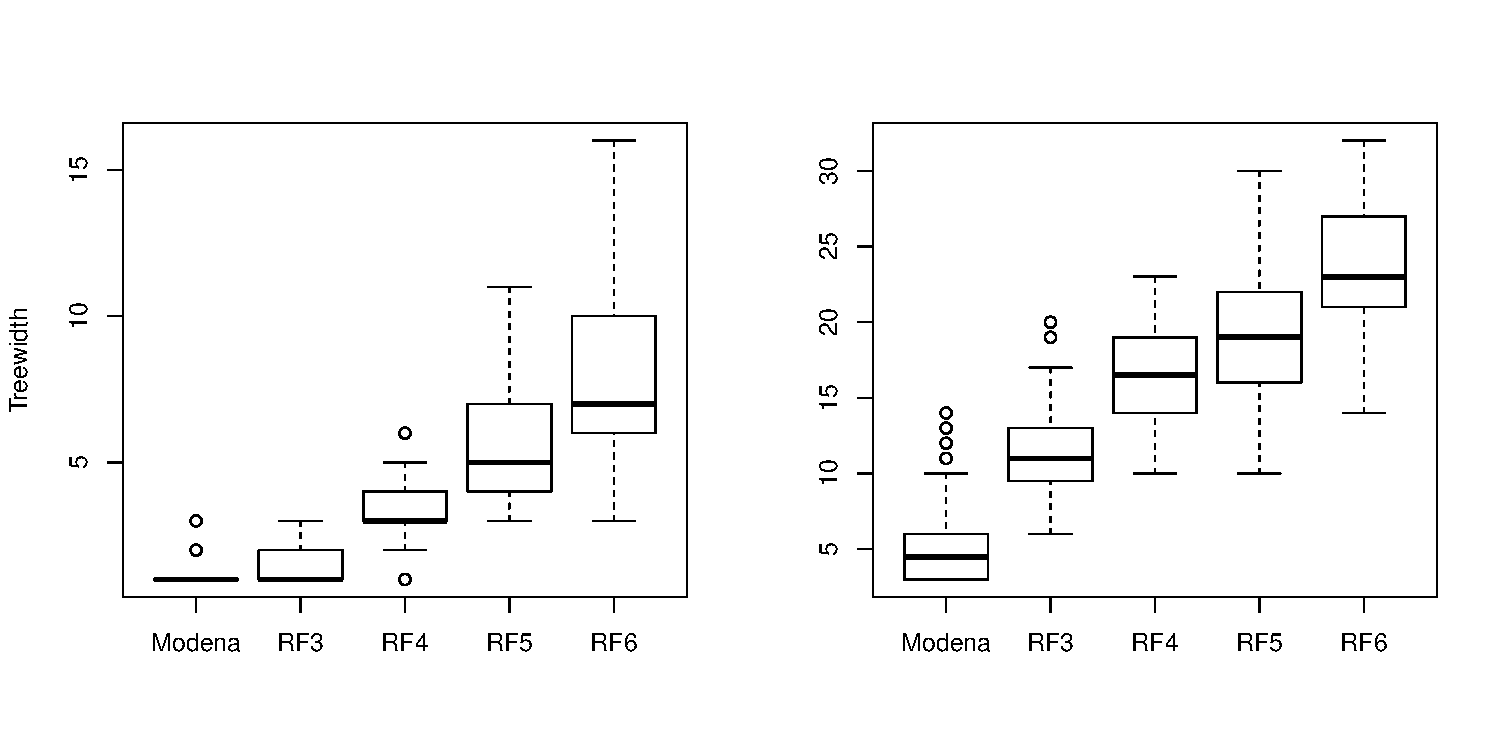
\includegraphics[width=0.9\textwidth]{Figs/td-widths}
  \vspace*{-24pt}
  \caption{Treewidths for multi-target RNA design instances of
    different complexity. Distributions of treewidths shown as boxplots for the base pair (left) and stacking model (right).}
  \label{fig:td-widths}
\end{figure}

\begin{figure}
  \hspace*{2cm}\textbf{Base pair model}\hspace{4.75cm}\textbf{Stacking model}\\[-28pt]
  \centering
  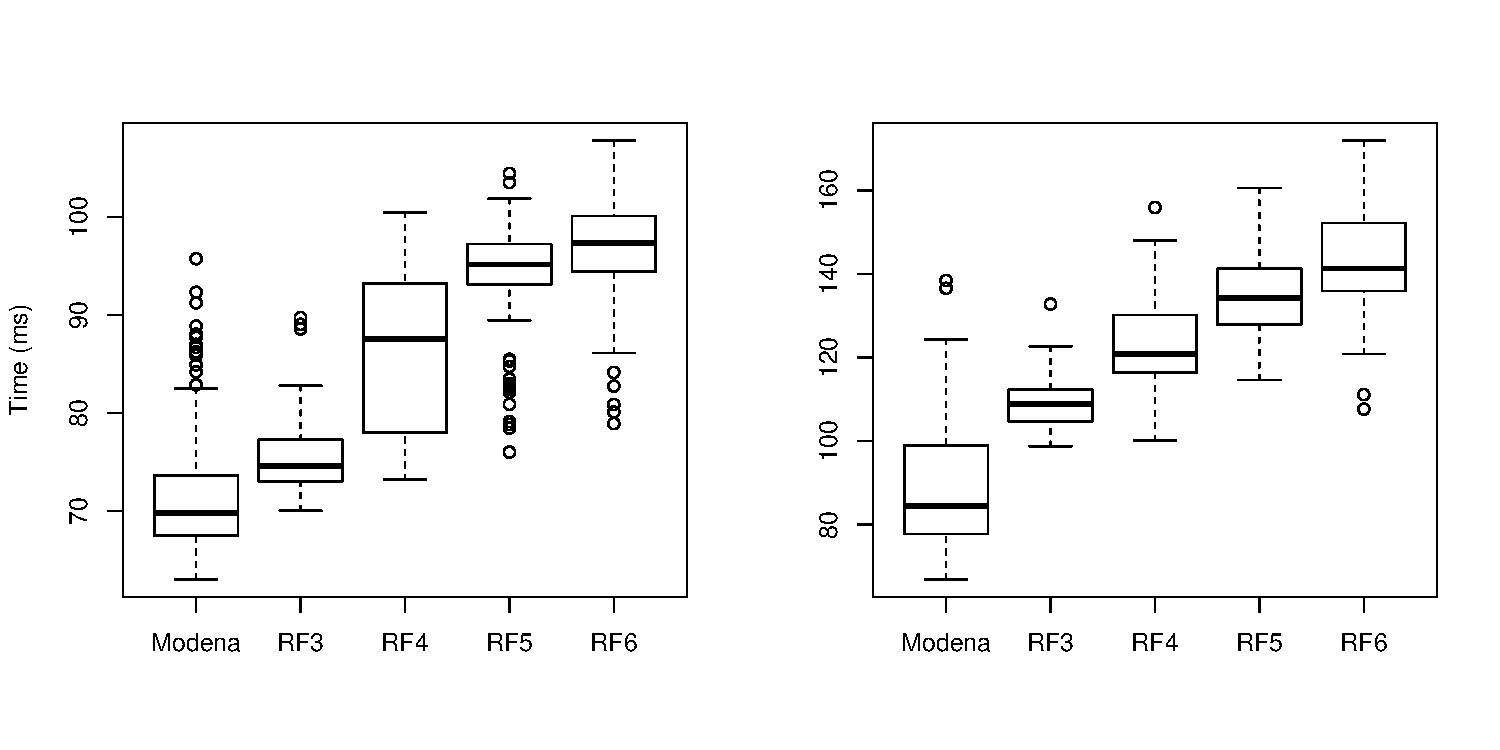
\includegraphics[width=0.9\textwidth]{Figs/td-times}
  \vspace*{-24pt}
  \caption{Computation time of tree decompositions for
    multi-target RNA design instances of different complexity.
    Distributions of times (in ms/instance) shown as boxplots for the base pair (left) and stacking model (right).}
  \label{fig:td-times}
\end{figure}


\begin{figure}[t!]
  %% the figure shows benchmark_inputs/RNAfold/3str/f3.100.0.inp
  \centering
  \verbatiminput{Figs/f3_100_0.txt}
  \includegraphicstop[width=0.6\textwidth]{Figs/td-example-basepair}%
  \includegraphicstop[width=0.35\textwidth]{Figs/td-example-stacking}
  \caption{Example instance from RF3 (top) with its tree decompositions in the base pair (left) and stacking model (right). The respective treewidths are 2 and 12.}
  \label{fig:td-example}
\end{figure}

\section{Expressing higher arity functions as cliques in the dependency graph}
\label{appsec:dependency-cliques}

Our implementation relies on external tools for the tree decomposition. Therefore it is not trivial that the weight functions (i.e. terms of the energy function) can be captured within the tree decompositions returned by a specific tool. In other words, it is not immediately clear how one can construct a cluster tree from an arbitrary tree decomposition for a given network. 

Fortunately, we can show that, as long as the network the arguments $\vars(f)$ of a function $f$ are materialized by a clique within the network $\network$, then there exists at least one node in the tree decomposition that contains $\vars(f)$, thus allowing the evaluation of $f$.
\begin{lemma}\label{lem:cliques}
Let $G=(V,E)$ be an undirected graph, and  $T,\chi$ be a tree decomposition for $G$. For each clique $C\subset V$, there exists a node $n\in T$ such that $C\subset\chi(v)$.
\end{lemma}
\begin{proof}
  \newcommand{\TransVars}[1]{{\rm tvars}(#1)}
  \newcommand{\Children}[1]{{\rm Children}(#1)}
  For the sake of simplicity, let us consider $T$ as rooted on an arbitrary node, inducing an orientation, and denote by $\TransVars{n}\in V$ the set of vertices found in a node $n$ or its descendants, namely
    $$\TransVars{n} = \chi(n) \bigcup_{n'\in\Children{n}} \TransVars{n'}.$$ 
  
  Now consider (one of) the deepest node(s) $n\in T$, such that $C\subset\TransVars{v}$. We are going to prove that $C\subset\chi(n)$, using contradiction, by showing that $C\not\subset\chi(n)$ implies that $T$ is not a tree decomposition. 
  
  Indeed, let us assume that $C\not\subset\chi(n)$, then there exists a node $v'\notin\chi(n)$ whose presence in $\TransVars{n}$ stems from its presence in some descendant of $n$. Let us denote by $n'\neq n$ the closest descendant of $n$ such that $v'\in\chi(n')$. Now, consider a node $v\in C$ such that $v\in \TransVars{v'}$ and $v\notin \TransVars{v'}$. Such a node always exists, otherwise $n'$, and not $n$, would be the deepest node such that $C\subset \TransVars{v'}$. From the definition of the tree decomposition, we know that neither $n'$ nor its descendants may contain $v$. On the other hand, none of the parents or siblings of $n'$ may contain $v'$. It follows that is no node $n''\in T$ whose vertex set $\chi(v'')$ includes, at the same time, $v$ and $v'$. Since both $v$ and $v'$ belong to a clique, one has $\{v,v'\}\in E$. The absence of a node in $T$ capturing an edge in $E$ contradicts our initial assumption that $T$ is tree decomposition for $G$.
  
  We conclude that $n$ is such that $C\not\subset\chi(n)$.
\end{proof}

This result implies that classic tree decomposition algorithms and, more importantly, implementations can be directly re-used to produce decompositions that capture energy models of arbitrary complexity, functions of arbitrary arity. Indeed, it suffices to add a clique, involving the parameters of the function, and Lemma~\ref{lem:cliques} guarantees that the tree decomposition will feature one node to which the function can be associated.


\section{Correctness of the FPT partition function algorithm}
\label{appsec:correctness}

\begin{theorem}[Correctness of Alg.~\ref{alg:pf}]
  \label{the:pfalgo-correctness}
  As computed by Alg.~\ref{alg:pf} for cluster tree $(T,\chi,\phi)$,
  the messages $\Message{u}{v}$, for all edges $u\to v\in T$, yield
  the partition functions of subtree of $u$ for the partial
  assignments $\val\in\assignments(\separator{u}{v})$, i.e. the
  messages satisfy
  \begin{equation}
   \Message{u}{v}[\val] = \sum_{\val'\in\assignments(\chi(T_r(u))-\separator{u}{v})} \quad
   \prod_{f\in\phi(T_r(u))} \exp(-\beta f[\val'|\val]),\label{eq:pfalgo-correct}
 \end{equation}
 where $\chi(T_r(u))$ denotes all $\chi$-assigned variables of nodes in $T_r(u)$;
 respectively $\phi(T_r(u))$; all $\phi$-assigned functions.
%
\end{theorem}

\begin{proof}
  Note that in more concise notation, Alg.~\ref{alg:pf} computes
  messages such that
\begin{equation}
  \Message{u}{v}[\val] := \sum_{\val'\in\assignments(\difference{u}{v})}\quad
  \prod_{f\in \phi(u) } \exp(-\beta f[\val'|\val]) \prod_{(w\to u) \in T} m_{w\to u}[\val'|\val].\label{eq:messages}
\end{equation}

Proof by induction on $T$. If $u$ is a leaf, $\chi(r) = \chi(T_r(u))$,
there are no messages sent to $u$, and $\phi(u) = \phi(T_r(u));$ implying
Eq.~$(\ref{eq:pfalgo-correct}).$
%
Otherwise, since the algorithm traverses edges in postorder, $u$ received from its children
$w_1,\dots,w_q$ the messages $m_{w_1\to u}, \dots, m_{w_q\to u}$, which satisfy Eq.~$(\ref{eq:pfalgo-correct})$ (induction hypothesis). Let $\val\in\assignments(\separator{u}{v})$; then, $\Message{u}{v}[\val]$ is computed by the algorithm according to Eq.~$(\ref{eq:messages})$. We rewrite as follows
\begin{align*}
  & \sum_{\val'\in\assignments(\difference{u}{v})}\quad
    \prod_{f\in \phi(u) } \exp(-\beta f[\val'|\val])
    \prod_{(w\to u) \in T} m_{w\to u}[\val'|\val]\\
  & = \sum_{\val'\in\assignments(\chi(u)-\separator{u}{v})}\quad
    \prod_{f\in \phi(u) } \exp(-\beta f[\val'|\val])
    \prod_{i=1}^q m_{w_i\to u}[\val'|\val]\\
  & =_{IH}
    \sum_{\val'\in\assignments(\chi(u)-\separator{u}{v})}\quad
    \prod_{f\in \phi(u) } \exp(-\beta f[\val'|\val])
    \prod_{i=1}^q \sum_{\val''\in\assignments(\chi(T_r(w_i))-\separator{w_i}{u})} \quad
    \prod_{f\in\phi(T_r(w_i))} \exp(-\beta f[\val'' | \val' | \val]) \\
& =_{*}
    \sum_{\val'\in\assignments(\chi(u)-\separator{u}{v})}\quad
  \sum_{\val''\in\assignments(\bigcup_{i=1}^q\chi(T_r(w_i))-\separator{w_i}{u})} \quad
  \prod_{f\in \phi(u) } \exp(-\beta f[\val'|\val])
  \prod_{f\in\phi(T_r(w_i))} \exp(-\beta f[\val'' | \val' | \val]) \\
  & =_{(**)} \sum_{\val'\in\assignments(\chi(T_r(u))-\separator{u}{v})}\quad
    \prod_{f\in \phi(T_r(u)) } \exp(-\beta f[\val'|\val])\\
\end{align*}
To see (*) and (**), we observe:
\begin{itemize}
\item The sets $\chi(u)-\separator{u}{v}$ and
  $\chi(T_r(w_i))-\separator{w_i}{u}$ are all disjoint due to
  Def.~\ref{def:treedecomp}, property 2. First, this property implies
  that any shared variable between the subtrees of $w_i$ and $w_j$
  must be in $\chi(w_i)$, $\chi(w_j)$ and $\chi(u)$, thus the
  variables of $\chi(T_r(w_i))-\separator{w_i}{u}$ are
  disjoint. Second, if a variable $\chi(T_r(w_i))$ occurs in
  $\chi(u)$, it must occur in $\chi(w_i)$ and consequently in $\separator{u}{v}$.
\item The union of the sets $\chi(u)-\separator{u}{v}$ and
  $\chi(T_r(w_i))-\separator{w_i}{u}$ is $\chi(T_r(u))-\separator{u}{v}).$
\end{itemize}

\end{proof}

\section{General complexity of the partition function computation by cluster tree elimination and generation of samples}
\label{appsec:algcomplexity}

\begin{proposition}
  \label{prop:general-complexity}
Given a cluster tree $(T,\chi,\phi)$, $T=(V,E)$ of the RNA design network $\network=(\X,\F)$ with treewidth $w$ and maximum separator size $s$, computing the partition function by Algorithm~\ref{alg:pf} takes $O((|F|+|V|)\cdot 4^{w+1})$ time and $O(|V| 4^s)$ space (for storing all messages). The sampling step has time complexity of $O((|F|+|V|)\cdot 4^D)$ per sample.
\end{proposition}

\begin{proof}[Proposition~\ref{prop:general-complexity}]
Let $d_u$ denote the degree of node $u$ in $T$, $s_u$ is the size of the separator between 
$u$ and its parent in $T$ rooted at $r$. For each node in the cluster tree, Alg.~\ref{alg:pf} computes one message by combining $(|\phi(u)|+d_u-1)$ functions, each time enumerating $4^{|\chi(u)|}$ combinations; Alg.~\ref{alg:sampling} computes $4^{|\chi{u}|-s_u}$ partition functions each time combining $(|\phi(u)|+d_u-1)$ functions.  $4^{|\chi(u)|}$ is bound by $4^{w+1}$ and $4^{|\chi{u}|-s_u}$ by $4^D$; moreover $\sum_{u\in V} (|\phi(u)|+d_u-1) = |F|+|V|-1$.
\end{proof}

\section{Parameters for the base pair and the stacking energy model}
\label{appsec:modelparameters}

We trained parameters for two RNA energy models to approximate the
Turner energy model, as implemented in the \Software{ViennaRNA}
package.  In the \Def{base pair model}, the total energy of a sequence $S$
for an RNA structure $R$ is given as sum of base pair energies, where
we consider six types of base pairs distinguishing by the bases A-U,
C-G or G-U (symmetrically) and between stacked and non-stacked base
pairs; here, we consider base pairs $(i,j)\in R$ \emph{stacked} iff
$(i+1,j-1)\in R$, otherwise \emph{non-stacked}. In the \Def{stacking model},
our features are defined by the stacks, i.e. pairs $(i,j)$ and
$(i+1,j-1)$ which both occur in $R$; we distinguish 18 types based on
$S_i,S_j,S_{i+1},S_{j-1}$ (i.e. all combinations that allow canonical
base pairs; the configurations $S_i,S_j,S_{i+1},S_{j-1}$ and
$S_{i+1},S_{j-1},S_j,S_i$ are symmetric).

Both models describe the energy assigned to a pair of sequence and
structure in linear dependency of the number of features and their
weights. We can thus train weights for linear predictors of the Turner
energy in both models.

For this purpose, we generated 5000 uniform random RNA sequences of
random lengths between 100 and 200. For each sample, we predict the
minimum free energy and corresponding structure using the ViennaRNA
package; then, we count the distinguished features (i.e., base pair or
stack types). The parameters are estimated fitting linear models
without intercept (\texttt{R} function \texttt{lm}). For both models,
\texttt{R} reports an adjusted R-squared value of 0.99. The resulting
parameters are reported in Tables~\ref{tab:basepairmodel} and
\ref{tab:stackingmodel}.

For validating the trained parameters, we generate a second
independent test set of random RNA sequences in the same
way. Figure~\ref{fig:training-cor} shows correlation plots for the
trained parameters in the base pair and stacking models for predicting
the Turner energies in the test set with respective correlations of
$0.95$ an $0.94$.

\begin{figure}
  \centering
  A)\includegraphicstop[width=0.4\textwidth,trim=0 0 0 50,clip]{Figs/basepaircor}
  B)\includegraphicstop[width=0.4\textwidth,trim=0 0 0 50,clip]{Figs/stackingcor}
  \caption{Validation of the trained parameters for the A) base pair
    model B) stacking model for predicting energies of the
    independently sampled sequences in the test set. We show
    correlation plots against the Turner energies reported by the
    ViennaRNA package.}
  \label{fig:training-cor}
\end{figure}

\begin{table}
  \centering
  \caption{Trained weights for the base pair energy model.} 
  \label{tab:basepairmodel}
  \begin{tabular}{c@{\quad}c@{\quad}c@{\quad}|@{\quad}c@{\quad}c@{\quad}c}
    \multicolumn{3}{c}{non-stacked} & \multicolumn{3}{c}{stacked}\\ 
    AU      & CG       & GU      & AU       & GC       & GU \\\hline
    1.26630 & -0.09070 & 0.78566 & -0.52309 & -2.10208 & -0.88474
  \end{tabular}
\end{table}

% GC_IN = -0.09070;
% AU_IN = 1.26630;
% GU_IN = 0.78566;
% GC_TERM = -2.10208;
% AU_TERM = -0.52309;
% GU_TERM = -0.88474;

\begin{table}
  \centering
  \caption{Trained weights for the stacking energy model (the rows specify $S_i,S_j$; the columns, $S_{i+1},S_{j-1}$; we do not show the symmetric weights).}
  \label{tab:stackingmodel}
  \begin{tabular}{c@{\quad}|@{\quad}c@{\quad}c@{\quad}c@{\quad}c@{\quad}c@{\quad}c@{\quad}c@{\quad}c}
       & AU & CG & GC & GU & UA & UG \\\hline
    AU &
-0.18826 &
-1.13291 &
-1.09787 &
-0.38606 &
-0.26510 &
-0.62086
    \\
    CG &
-1.11752 &
-2.23740 &
-1.89434 &
-1.22942 &
-1.10548 &
-1.44085
    \\
    GU &
-0.55066 &
-1.26209 &
-1.58478 &
-0.72185 &
-0.49625 &
-0.68876
    \\
  \end{tabular}
\end{table}

\section{Monotonicity of the partial derivatives within weight calibration}
\label{sec:weight_derivatives}
%
In weighted distributions, one witnesses a fairly predictable impact of the variation of any weight $\pi_\ell$ over the expected value $\mathbb{E}(E_\ell\mid \pmb{\pi})$, $\pmb{\pi}:= (\pi_1\cdots\pi_k)$, of the free energy $E_\ell$ of structure $\ell$.  Let us  first remind the probability of a sequence $S$ in the weighted distribution
\begin{align*} 
  \mathcal{B}_{\pmb{\pi}}(S) &= \prod_{i=1}^{k} \pi_i^{-E_i(S)}, &
  \partfun{\pmb{\pi}}&=\sum_{S'}\mathcal{B}_{\pmb{\pi}}(S') &
    \text{and}& &
  \mathbb{P}(S\mid \pmb{\pi}) &= \frac{\mathcal{B}_{\pmb{\pi}}(S)}{\partfun{\pmb{\pi}}}.
  \end{align*}
  
Remind also the definition of the expectation of $E_\ell(S)$, for $S$ a Boltzmann-distributed sequence:
$$\mathbb{E}(E_\ell\mid \pmb{\pi}) = \sum_S E_\ell(S)\cdot \mathbb{P}(S\mid \pmb{\pi}).$$

We first remark that the partial derivative of $\mathcal{B}$ yields
\begin{align*} 
  \frac{\partial \mathcal{B}_{\pmb{\pi}}(S)}{\partial \pi_\ell} = -E_\ell(S)\cdot \pi_\ell^{-E_\ell(S)-1}\prod_{\substack{i=1\\i\neq \ell}}^{k} \pi_i^{-E_i(S)} = \frac{-E_\ell(S)}{\pi_\ell}\cdot\mathcal{B}_{\pmb{\pi}}(S) = -E_\ell(S)\cdot \mathbb{P}(S\mid \pmb{\pi})\cdot \frac{\partfun{\pmb{\pi}}}{\pi_\ell }
\end{align*}
while the partial derivative of $\mathcal{Z}$ gives 
\begin{align*} 
  \frac{\partial \partfun{\pmb{\pi}}(S)}{\partial \pi_\ell} = \sum_{S'} -E_\ell(S')\cdot \mathbb{P}(S'\mid \pmb{\pi})\cdot \frac{\partfun{\pmb{\pi}}}{\pi_\ell }= -\mathbb{E}(E_\ell\mid \pmb{\pi})\cdot \frac{\partfun{\pmb{\pi}}}{\pi_\ell}.
\end{align*}
From these expressions, we conclude that
\begin{align*} 
  \frac{\partial \mathbb{E}(E_\ell\mid \pmb{\pi})}{\partial \pi_\ell} &= \sum_S E_\ell(S)\cdot\frac{\partial \mathbb{P}(S\mid \pmb{\pi})}{\partial \pi_\ell}\\
  %
  & = \sum_S E_\ell(S)\left(\frac{\frac{\partial \mathcal{B}_{\pmb{\pi}}(S)}{\partial \pi_\ell}}{\mathcal{Z}_{\pmb{\pi}}} - \frac{\frac{\partial \mathcal{Z}_{\pmb{\pi}}}{\partial \pi_\ell}\cdot\mathcal{B}_{\pmb{\pi}}(S)}{\mathcal{Z}_{\pmb{\pi}}^2}\right)\\
  %
  & = \sum_S E_\ell(S)\left(\frac{-E_\ell(S)\cdot \mathbb{P}(S\mid \pmb{\pi})\cdot \frac{\mathcal{Z}_{\pmb{\pi}}}{\pi_\ell }}{\mathcal{Z}_{\pmb{\pi}}} + \frac{\mathbb{E}(E_\ell\mid \pmb{\pi})\cdot \frac{\mathcal{Z}_{\pmb{\pi}}}{\pi_\ell}\cdot\mathcal{B}_{\pmb{\pi}}(S)}{\mathcal{Z}_{\pmb{\pi}}^2}\right)\\
  %
  & = \sum_S - \frac{E_\ell(S)^2\cdot\mathbb{P}(S\mid \pmb{\pi})}{\pi_\ell} + \frac{\mathbb{E}(E_\ell\mid \pmb{\pi})}{\pi_\ell}\sum_S E_\ell(S)\cdot \mathbb{P}(S\mid \pmb{\pi})\\
  & = -\frac{\mathbb{E}(E_\ell^2\mid \pmb{\pi}) - \mathbb{E}(E_\ell\mid \pmb{\pi})^2}{\pi_\ell}
\end{align*}
In the numerator of the above expression, one recognizes the variance of the distribution of $E_\ell$.
Remark that a variance is always non-negative and, in our case, also strictly positive for $\pmb{\pi}$, $\pi_\ell>0$, as soon as there exist at least two distinct sequences $S$ and $S'$ such that $E_\ell(S)\neq E_\ell(S')$.
Moreover, weights are always positive so the partial derivative in $\pi_\ell$ is always positive. Ultimately, it is always possible to increase (resp. decrease) the expected free energy of a structure by simply decreasing (resp. increasing) its weight, supporting our weight optimization procedure.
\newpage
\section{Detailed result of quality analysis}\label{sec:validity}
N/A values correspond to data that could not be obtained by the time of this submission for two main reasons: In the case of the initial sampling (left columns), they correspond to instances which, in conjunction with an expressive energy model, resulted in very high tree-width, leading to unreasonable memory requirements incompatible with our available computing resources; The case of missing values after optimization  (right columns), they indicate situations where the initial optimization took too long ($\approx$ 1 day) and was killed.
\subsection{RNAtabupath (2 structures)}
{\relsize{-1}
\begin{longtable}{@{}cr@{\hspace{1em}}r@{\hspace{1em}}r@{\hspace{1em}}r@{\hspace{1em}}r@{\hspace{2em}}r@{\hspace{1em}}r@{\hspace{1em}}r@{\hspace{1em}}r@{\hspace{1em}}r@{}}
&\multicolumn{2}{c}{Boltzmann}&\multicolumn{2}{l}{Uniform}&&\multicolumn{2}{l}{\begin{minipage}[b]{1.8cm} Boltzmann\\Optimized\end{minipage}}&\multicolumn{2}{l}{\begin{minipage}[b]{1.8cm} Uniform\\Optimized\end{minipage}}&\\ \toprule
Name&Mean&StDev&Mean&StDev&\%Gain&Mean&StDev&Mean&StDev&\%Gain\\ \midrule
alpha\_operon&17.18&4.18&25.86&5.97&51&2.12&0.81&2.36&0.88&11\\
amv&14.37&2.90&27.26&5.65&90&3.67&0.90&4.27&1.08&16\\
attenuator&10.74&3.04&21.44&4.77&100&1.39&0.55&1.81&0.80&30\\
dsrA&11.77&2.58&18.23&4.62&55&3.71&0.94&3.80&0.95& 2\\
hdv&22.08&4.88&35.48&6.68&61&3.63&1.16&4.57&1.48&26\\
hiv&41.22&6.74&73.00&9.40&77&16.87&3.45&29.89&5.36&77\\
ms2&13.35&3.73&19.79&4.55&48&2.41&0.76&2.66&0.97&10\\
rb1&17.70&4.35&37.38&7.14&111&2.64&0.90&3.82&1.31&45\\
rb2&16.63&4.16&25.17&5.85&51&2.75&0.86&3.07&0.97&12\\
rb3&22.47&4.71&41.18&7.09&83&3.79&1.01&5.05&1.52&33\\
rb4&26.15&4.30&47.89&6.80&83&10.57&&11.80&1.82&12\\
rb5&30.52&5.45&54.24&7.76&78&6.10&1.97&9.22&2.78&51\\
ribD&49.84&7.01&81.27&9.07&63&20.47&3.17&31.01&4.47&51\\
s15&11.00&2.97&18.37&4.53&67&1.96&0.64&2.12&0.77& 8\\
sbox&25.05&4.84&50.03&8.04&100&6.34&1.49&8.90&2.19&40\\
spliced&9.65&2.98&17.60&4.39&82&2.13&0.44&2.41&0.59&13\\
sv11&20.98&4.66&36.83&6.91&76&N/A&N/A&4.20&1.12&N/A\\
thim&29.35&5.39&48.32&6.95&65&8.69&1.90&12.12&2.54&39\\
\midrule
Average&21.67&4.38&37.74&6.45&74&5.84&1.31&7.95&1.76&28\\\bottomrule
\end{longtable}}
\subsection{RNAdesign (3 structures)}
{\relsize{-1}
\begin{longtable}{@{}cr@{\hspace{1em}}r@{\hspace{1em}}r@{\hspace{1em}}r@{\hspace{1em}}r@{\hspace{2em}}r@{\hspace{1em}}r@{\hspace{1em}}r@{\hspace{1em}}r@{\hspace{1em}}r@{}}
&\multicolumn{2}{c}{Boltzmann}&\multicolumn{2}{l}{Uniform}&&\multicolumn{2}{l}{\begin{minipage}[b]{1.8cm} Boltzmann\\Optimized\end{minipage}}&\multicolumn{2}{l}{\begin{minipage}[b]{1.8cm} Uniform\\Optimized\end{minipage}}&\\ \toprule
Name&Mean&StDev&Mean&StDev&\%Gain&Mean&StDev&Mean&StDev&\%Gain\\\midrule
sq100&20.67&4.90&31.78&5.46&54&5.81&1.53&8.33&1.92&43\\
sq10&19.91&5.24&26.62&5.59&34&3.50&0.81&3.88&0.94&11\\
sq11&19.38&4.81&27.76&5.69&43&2.81&0.77&3.31&0.89&18\\
sq12&17.19&3.62&22.62&4.98&32&2.70&0.65&2.79&0.68& 3\\
sq13&18.54&3.95&29.95&5.56&62&10.24&2.18&16.63&3.13&62\\
sq14&21.49&4.23&37.82&5.55&76&7.25&1.63&9.90&2.10&37\\
sq15&21.91&3.78&36.32&5.13&66&11.15&1.75&15.49&2.34&39\\
sq16&15.99&4.22&27.70&5.58&73&2.51&0.69&2.96&0.94&18\\
sq17&20.71&3.72&33.62&5.33&62&5.83&1.08&7.36&1.49&26\\
sq18&19.64&3.91&35.26&5.13&80&5.83&1.41&7.97&2.00&37\\
sq19&14.78&3.33&28.64&5.34&94&3.84&0.77&4.66&1.04&21\\
sq1&14.85&3.84&21.89&5.48&47&2.02&0.65&2.20&0.69& 9\\
sq20&17.39&3.82&27.90&4.93&60&3.93&1.04&5.18&1.48&32\\
sq21&21.64&3.94&36.27&5.16&68&8.28&1.82&11.41&2.40&38\\
sq22&17.65&4.13&31.57&5.45&79&5.66&1.51&10.02&2.50&77\\
sq23&19.44&3.66&32.38&5.40&67&12.05&1.85&18.69&3.18&55\\
sq24&18.01&4.01&27.92&5.30&55&3.59&0.93&4.25&1.10&19\\
sq25&17.54&5.20&26.65&6.11&52&1.35&0.34&1.45&0.40& 7\\
sq26&17.63&4.47&24.46&5.64&39&3.11&0.62&3.38&0.68& 9\\
sq27&17.93&3.61&28.51&5.30&59&7.55&1.49&10.96&2.38&45\\
sq28&14.78&3.71&29.35&5.99&99&2.32&0.49&2.66&0.62&15\\
sq29&17.61&3.72&26.95&5.08&53&4.44&0.98&5.22&1.21&18\\
sq2&22.43&4.19&37.25&5.15&66&10.34&1.71&14.32&2.35&39\\
sq30&19.11&4.04&31.75&5.54&66&6.06&1.61&8.99&2.19&48\\
sq31&19.97&3.87&31.92&5.20&60&5.12&1.19&6.34&1.55&24\\
sq32&21.96&4.00&31.65&5.23&44&5.24&1.29&6.84&1.76&31\\
sq33&15.11&4.30&22.75&5.52&51&1.78&0.43&2.08&0.63&17\\
sq34&25.00&4.17&37.46&5.03&50&12.46&1.84&18.73&2.57&50\\
sq35&19.25&4.12&32.72&5.35&70&5.90&1.25&7.96&1.82&35\\
sq36&12.77&2.91&26.76&5.39&110&3.19&0.77&3.61&0.94&13\\
sq37&18.71&3.88&32.44&5.62&73&3.24&0.90&4.21&1.25&30\\
sq38&14.55&3.56&29.02&5.29&99&2.79&0.86&3.70&1.22&33\\
sq39&22.75&3.95&33.06&4.98&45&9.20&1.76&11.87&2.33&29\\
sq3&20.38&4.07&36.86&5.60&81&4.69&1.19&6.30&1.72&34\\
sq40&19.46&4.35&31.76&5.41&63&4.05&0.94&4.96&1.19&23\\
sq41&14.41&3.46&27.85&5.57&93&3.33&0.71&3.91&0.88&17\\
sq42&18.67&3.87&35.20&5.55&89&5.32&1.24&6.96&1.56&31\\
sq43&17.32&3.97&31.63&5.38&83&3.53&0.89&4.27&1.15&21\\
sq44&19.37&3.84&31.75&5.09&64&5.52&1.29&7.26&1.60&31\\
sq45&18.53&4.77&27.40&5.53&48&2.54&0.67&2.84&0.74&12\\
sq46&17.92&3.80&28.83&5.09&61&4.45&0.90&5.41&1.20&22\\
sq47&15.09&3.78&28.23&5.82&87&3.02&0.78&3.45&0.85&14\\
sq48&18.90&4.23&36.27&5.78&92&4.69&1.08&6.71&1.67&43\\
sq49&20.13&4.69&27.24&5.39&35&3.15&0.76&3.66&0.95&16\\
sq4&19.31&4.69&29.25&5.34&51&2.36&0.79&3.24&1.15&37\\
sq50&17.01&3.92&28.43&5.35&67&3.15&0.73&3.54&0.86&12\\
sq51&22.18&4.14&36.07&5.20&63&11.56&1.79&16.57&2.88&43\\
sq52&19.36&3.93&31.04&5.20&60&11.04&2.21&16.25&3.04&47\\
sq53&13.78&3.72&24.48&5.46&78&1.65&0.39&1.88&0.53&14\\
sq54&18.07&3.59&33.99&5.57&88&8.15&1.57&12.35&2.59&51\\
sq55&21.93&4.68&30.11&5.21&37&4.59&0.82&5.43&1.13&18\\
sq56&17.83&3.90&31.69&5.46&78&4.22&0.75&4.84&0.93&15\\
sq57&16.30&3.97&28.48&5.45&75&1.96&0.58&2.28&0.71&16\\
sq58&12.74&2.86&32.97&5.80&159&3.77&0.82&4.89&1.22&29\\
sq59&20.44&4.54&33.02&5.57&62&6.05&1.50&8.34&2.08&38\\
sq5&9.97&2.72&17.94&4.93&80&1.29&0.33&1.41&0.39& 9\\
sq60&22.64&4.85&36.86&5.46&63&6.90&1.62&11.07&2.33&60\\
sq61&14.45&3.78&30.82&6.03&113&3.07&0.76&3.83&1.01&25\\
sq62&21.08&5.02&35.27&5.35&67&9.76&1.67&16.93&2.79&73\\
sq63&13.44&3.60&27.20&5.63&102&1.58&0.36&1.85&0.53&17\\
sq64&19.21&3.87&34.88&5.24&82&6.10&1.53&9.45&2.29&55\\
sq65&19.33&4.53&27.51&5.15&42&13.95&2.94&19.40&3.61&39\\
sq66&18.18&3.70&30.79&5.12&69&6.93&1.42&10.05&2.03&45\\
sq67&20.63&3.41&37.06&5.18&80&16.11&1.97&27.21&3.40&69\\
sq68&23.09&4.33&33.33&5.08&44&N/A&N/A&9.23&1.94&N/A\\
sq69&18.79&3.58&35.06&5.21&87&10.77&1.94&18.38&3.00&71\\
sq6&20.32&3.77&38.48&5.48&89&5.55&1.32&8.63&2.04&56\\
sq70&13.59&3.31&31.06&5.52&129&2.59&0.80&3.80&1.17&47\\
sq71&20.07&4.05&32.71&5.39&63&5.57&1.06&6.61&1.30&19\\
sq72&15.02&3.22&24.48&4.94&63&2.02&0.57&2.49&0.84&23\\
sq73&14.88&3.74&28.44&5.56&91&2.34&0.69&3.10&1.04&32\\
sq74&17.80&4.10&30.13&5.30&69&4.12&0.79&5.03&1.04&22\\
sq75&19.66&4.05&31.19&5.19&59&5.63&1.26&7.52&1.70&34\\
sq76&19.91&3.84&32.44&5.12&63&9.12&1.92&13.89&2.39&52\\
sq77&18.69&3.46&34.83&5.21&86&6.01&1.25&8.61&1.75&43\\
sq78&18.28&3.48&32.94&6.01&80&5.39&1.12&7.07&1.51&31\\
sq79&21.57&4.71&30.73&5.47&42&13.10&2.89&17.86&3.45&36\\
sq7&20.28&3.76&32.95&5.41&63&5.51&1.70&6.68&1.90&21\\
sq80&15.62&3.92&28.29&5.30&81&1.85&0.53&2.41&0.88&30\\
sq81&21.24&4.57&29.92&5.44&41&3.74&0.95&4.67&1.33&25\\
sq82&8.85&2.35&19.89&5.36&125&1.39&0.21&1.47&0.28& 6\\
sq83&14.13&3.60&28.92&5.45&105&2.77&0.76&3.52&1.01&27\\
sq84&15.60&3.98&24.12&5.26&55&2.54&0.47&2.85&0.65&12\\
sq85&15.56&3.39&26.09&5.18&68&2.19&0.62&2.70&0.82&23\\
sq86&21.54&4.95&34.21&5.77&59&4.66&1.21&5.92&1.51&27\\
sq87&16.45&3.85&32.65&5.81&98&3.50&0.62&4.14&0.86&18\\
sq88&20.05&5.09&33.45&5.86&67&2.50&0.72&3.17&0.99&27\\
sq89&14.77&4.20&26.15&5.59&77&1.79&0.50&2.01&0.62&13\\
sq8&15.85&4.14&30.34&6.02&91&2.85&0.79&3.85&1.15&35\\
sq90&15.25&3.99&29.83&5.80&96&2.10&0.64&2.90&1.06&38\\
sq91&17.29&3.93&27.19&5.08&57&3.69&1.11&4.48&1.31&21\\
sq92&19.06&3.57&33.07&5.34&74&4.77&1.11&6.83&1.78&43\\
sq93&19.48&4.11&29.17&5.65&50&3.29&0.80&3.86&1.03&17\\
sq94&14.72&3.21&27.05&5.43&84&3.98&0.77&4.66&0.98&17\\
sq95&17.60&3.72&33.42&5.38&90&12.86&2.20&22.76&3.84&77\\
sq96&15.35&3.84&31.62&5.68&106&2.69&0.67&3.52&1.02&31\\
sq97&18.28&3.89&29.22&5.03&60&4.31&1.13&5.32&1.42&23\\
sq98&18.84&4.57&29.30&5.42&56&2.78&0.73&3.59&0.97&29\\
sq99&19.74&4.19&30.95&5.28&57&3.94&0.98&4.89&1.33&24\\
sq9&17.30&4.26&26.15&5.72&51&1.66&0.44&1.79&0.55&8\\
\midrule
Average&21.67&4.38&37.74&6.45&74&5.84&1.31&7.95&1.76&28\\\bottomrule
\end{longtable}}
\subsection{RNAdesign (4 structures)}
{\relsize{-1}
\begin{longtable}{@{}cr@{\hspace{1em}}r@{\hspace{1em}}r@{\hspace{1em}}r@{\hspace{1em}}r@{\hspace{2em}}r@{\hspace{1em}}r@{\hspace{1em}}r@{\hspace{1em}}r@{\hspace{1em}}r@{}}
&\multicolumn{2}{c}{Boltzmann}&\multicolumn{2}{l}{Uniform}&&\multicolumn{2}{l}{\begin{minipage}[b]{1.8cm} Boltzmann\\Optimized\end{minipage}}&\multicolumn{2}{l}{\begin{minipage}[b]{1.8cm} Uniform\\Optimized\end{minipage}}&\\ \toprule
Name&Mean&StDev&Mean&StDev&\%Gain&Mean&StDev&Mean&StDev&\%Gain\\\midrule
sq100&21.70&4.41&33.19&4.93&53&12.52&2.62&17.14&3.10&37\\
sq10&20.66&5.16&27.00&5.24&31&N/A&N/A&8.02&2.05&N/A\\
sq11&22.23&4.23&30.73&5.31&38&6.09&1.21&7.70&1.70&26\\
sq12&18.30&3.55&23.38&4.93&28&3.75&0.53&3.94&0.64& 5\\
sq13&21.01&3.57&31.66&4.93&51&15.63&1.69&21.61&2.69&38\\
sq14&22.44&3.16&39.77&5.28&77&17.56&2.21&25.04&3.21&43\\
sq15&22.66&3.72&36.31&5.01&60&17.45&2.38&26.80&3.34&54\\
sq16&18.22&4.12&28.54&5.33&57&3.27&0.74&3.78&0.90&16\\
sq17&23.04&4.01&35.87&5.28&56&12.76&2.54&18.43&2.86&44\\
sq18&21.20&3.49&35.78&5.39&69&8.15&1.47&10.75&2.02&32\\
sq19&15.36&2.73&32.12&4.95&109&13.22&1.73&23.64&3.41&79\\
sq1&15.14&3.83&22.32&5.28&47&2.55&0.56&2.66&0.56& 4\\
sq20&16.75&3.09&29.25&4.74&75&9.26&1.67&13.40&2.41&45\\
sq21&23.98&3.72&38.18&5.14&59&16.15&2.10&23.31&3.16&44\\
sq22&20.38&3.81&32.90&5.12&61&8.42&1.44&12.39&2.03&47\\
sq23&18.39&3.36&32.82&5.34&78&12.07&1.93&19.58&3.26&62\\
sq24&20.05&4.10&29.72&5.29&48&5.40&1.15&7.28&1.68&35\\
sq25&21.48&5.35&28.83&5.78&34&2.95&0.66&3.30&0.77&12\\
sq26&20.83&4.63&27.39&5.25&32&4.20&0.76&4.80&0.96&14\\
sq27&17.14&3.48&29.41&5.24&72&7.58&1.45&11.67&2.34&54\\
sq28&23.50&4.48&33.84&6.07&44&5.59&1.03&6.69&1.39&20\\
sq29&18.14&3.65&27.22&4.85&50&5.54&0.92&6.26&1.17&13\\
sq2&N/A&N/A&N/A&N/A&N/A&N/A&N/A&N/A&N/A&N/A\\
sq30&19.40&3.76&32.40&4.95&67&8.89&1.56&12.39&2.19&39\\
sq31&24.97&3.80&32.68&5.19&31&8.77&1.18&13.05&2.15&49\\
sq32&19.62&3.76&31.03&4.97&58&5.50&1.29&7.57&1.71&38\\
sq33&19.51&4.25&27.65&5.12&42&4.23&0.91&5.37&1.16&27\\
sq34&25.60&3.50&37.58&4.90&47&13.41&1.77&20.62&2.68&54\\
sq35&21.87&3.93&35.50&5.73&62&9.66&1.56&13.80&2.31&43\\
sq36&11.65&2.59&26.29&5.48&126&3.33&0.60&3.86&0.90&16\\
sq37&25.80&4.48&36.19&4.90&40&15.84&2.03&23.46&2.85&48\\
sq38&17.74&3.43&32.11&5.14&81&4.95&0.93&6.20&1.38&25\\
sq39&21.54&3.83&32.74&5.21&52&9.79&1.81&13.10&2.29&34\\
sq3&20.19&4.06&39.87&5.23&97&14.60&2.26&26.21&3.32&79\\
sq40&18.68&4.18&33.41&5.62&79&4.32&0.92&5.49&1.30&27\\
sq41&15.86&3.46&30.06&5.30&89&5.56&0.94&6.59&1.17&19\\
sq42&21.79&3.25&38.72&5.11&78&N/A&N/A&23.27&3.45&N/A\\
sq43&23.21&3.99&33.89&5.33&46&7.27&1.30&9.08&1.76&25\\
sq44&21.65&3.59&33.47&4.99&55&8.04&1.42&10.91&1.97&36\\
sq45&19.01&4.79&27.79&5.58&46&3.45&0.65&3.81&0.83&10\\
sq46&20.08&3.60&30.69&4.89&53&7.68&1.30&9.96&1.69&30\\
sq47&17.29&3.73&29.94&5.26&73&4.52&1.03&5.24&1.20&16\\
sq48&28.78&4.03&38.24&5.57&33&16.87&1.76&25.52&3.19&51\\
sq49&19.19&4.75&27.33&5.42&42&3.14&0.73&3.66&0.86&17\\
sq4&19.71&4.46&29.44&5.30&49&3.35&0.87&4.25&1.18&27\\
sq50&19.36&4.11&30.60&5.49&58&4.99&0.79&5.71&0.98&14\\
sq51&N/A&N/A&38.68&5.02&N/A&N/A&N/A&27.99&2.48&N/A\\
sq52&21.40&3.37&33.80&5.43&58&16.30&2.43&25.10&3.67&54\\
sq53&15.81&3.50&28.75&5.32&82&4.29&1.05&6.22&1.53&45\\
sq54&18.16&3.45&35.10&4.86&93&15.32&2.23&26.27&3.37&71\\
sq55&22.47&4.43&31.94&5.15&42&11.05&2.41&15.19&2.98&37\\
sq56&21.11&4.12&35.25&5.93&67&12.27&2.00&18.68&2.97&52\\
sq57&18.94&3.91&30.86&5.51&63&3.69&0.71&4.51&0.90&22\\
sq58&19.68&2.97&35.80&5.41&82&9.78&1.44&16.76&2.66&71\\
sq59&20.35&3.75&33.08&5.20&63&17.24&2.82&24.28&3.93&41\\
sq5&11.60&2.54&19.61&5.12&69&1.92&0.35&2.12&0.49&11\\
sq60&21.97&4.37&38.39&5.44&75&17.44&2.44&29.57&3.89&70\\
sq61&19.07&3.46&34.14&5.24&79&6.90&1.33&10.30&1.97&49\\
sq62&25.71&5.09&34.50&4.88&34&12.33&1.94&17.33&2.62&41\\
sq63&17.21&3.45&30.71&5.37&78&5.49&1.36&7.38&1.84&34\\
sq64&19.89&3.52&35.51&4.96&79&14.00&2.12&22.04&3.12&57\\
sq65&18.69&4.06&29.18&5.34&56&12.55&2.26&17.63&2.94&41\\
sq66&17.50&3.40&30.59&5.16&75&8.71&1.62&13.67&2.43&57\\
sq67&22.63&4.21&36.73&5.06&62&17.17&2.21&26.90&3.34&57\\
sq68&N/A&N/A&35.00&5.13&N/A&N/A&N/A&17.96&2.39&N/A\\
sq69&N/A&N/A&36.07&4.91&N/A&N/A&N/A&24.53&2.08&N/A\\
sq6&22.32&3.77&40.27&5.41&80&6.25&1.39&9.46&2.08&51\\
sq70&16.97&4.07&31.84&5.51&88&3.64&0.88&5.09&1.32&40\\
sq71&19.34&4.07&31.81&5.24&64&5.09&0.95&6.26&1.20&23\\
sq72&16.60&3.01&29.22&4.92&76&6.20&1.18&7.67&1.57&24\\
sq73&18.64&3.44&30.86&5.16&66&12.54&2.35&21.15&4.05&69\\
sq74&17.24&3.88&31.19&5.47&81&13.12&3.31&21.49&4.11&64\\
sq75&18.44&3.60&31.25&5.19&70&7.24&1.37&11.19&2.21&55\\
sq76&20.76&3.38&33.74&4.94&63&16.90&2.38&25.18&3.38&49\\
sq77&21.92&3.29&35.83&5.26&63&10.59&1.63&13.96&2.25&32\\
sq78&23.60&3.17&36.23&5.47&54&19.14&2.52&26.07&3.61&36\\
sq79&24.77&4.43&32.49&5.23&31&18.07&2.89&23.78&3.64&32\\
sq7&19.94&3.54&32.78&5.29&64&5.37&1.65&6.59&1.89&23\\
sq80&18.63&3.88&29.75&5.27&60&2.87&0.64&3.64&1.01&26\\
sq81&23.57&3.63&36.02&5.24&53&17.71&2.20&25.76&3.17&45\\
sq82&13.21&3.25&25.45&5.00&93&3.05&0.67&4.06&1.00&33\\
sq83&14.37&3.21&31.96&5.41&122&3.86&0.84&5.55&1.31&44\\
sq84&19.05&3.89&29.35&5.00&54&5.21&0.99&6.38&1.32&23\\
sq85&17.32&3.91&30.80&5.43&78&10.61&2.09&17.53&2.93&65\\
sq86&25.19&4.04&36.79&5.66&46&9.04&1.93&14.14&2.62&56\\
sq87&16.91&3.89&32.84&5.34&94&4.94&0.79&6.08&1.18&23\\
sq88&22.92&4.99&35.87&5.65&56&5.22&1.00&6.58&1.30&26\\
sq89&17.52&3.91&29.24&5.45&67&4.14&0.86&4.83&1.11&17\\
sq8&25.56&4.49&33.42&5.21&31&N/A&N/A&12.55&2.05&N/A\\
sq90&18.67&3.62&33.21&5.33&78&5.40&0.98&7.26&1.62&34\\
sq91&18.00&3.83&26.82&4.85&49&8.01&1.72&11.08&2.41&38\\
sq92&20.51&3.28&37.62&4.84&N/A&17.62&2.17&29.08&3.47&65\\
sq93&22.63&4.66&33.40&5.25&48&11.43&2.16&16.37&3.00&43\\
sq94&14.71&3.25&28.06&5.39&91&3.81&0.72&4.51&0.97&18\\
sq95&N/A&N/A&36.93&5.11&N/A&N/A&N/A&23.98&2.67&N/A\\
sq96&17.20&3.70&33.01&5.46&92&5.98&1.20&8.09&1.71&35\\
sq97&19.78&3.85&30.01&5.09&52&6.05&1.25&7.45&1.60&23\\
sq98&21.39&4.33&31.13&5.16&46&4.77&0.77&5.67&1.03&19\\
sq99&20.33&4.39&29.97&5.07&47&4.05&1.07&4.95&1.28&22\\
sq9&18.86&4.22&29.51&5.22&56&3.93&0.88&5.06&1.35&29\\
\\\midrule
Average&19.94&3.84&32.29&5.24&63&8.77&1.48&13.13&2.13&37\\ \bottomrule
\end{longtable}}


\end{document}


